% Options for packages loaded elsewhere
% Options for packages loaded elsewhere
\PassOptionsToPackage{unicode}{hyperref}
\PassOptionsToPackage{hyphens}{url}
\PassOptionsToPackage{dvipsnames,svgnames,x11names}{xcolor}
%
\documentclass[
  12pt,
  letterpaper,
]{article}
\usepackage{xcolor}
\usepackage[margin=.5in]{geometry}
\usepackage{amsmath,amssymb}
\setcounter{secnumdepth}{5}
\usepackage{iftex}
\ifPDFTeX
  \usepackage[T1]{fontenc}
  \usepackage[utf8]{inputenc}
  \usepackage{textcomp} % provide euro and other symbols
\else % if luatex or xetex
  \usepackage{unicode-math} % this also loads fontspec
  \defaultfontfeatures{Scale=MatchLowercase}
  \defaultfontfeatures[\rmfamily]{Ligatures=TeX,Scale=1}
\fi
\usepackage{lmodern}
\ifPDFTeX\else
  % xetex/luatex font selection
\fi
% Use upquote if available, for straight quotes in verbatim environments
\IfFileExists{upquote.sty}{\usepackage{upquote}}{}
\IfFileExists{microtype.sty}{% use microtype if available
  \usepackage[]{microtype}
  \UseMicrotypeSet[protrusion]{basicmath} % disable protrusion for tt fonts
}{}
\makeatletter
\@ifundefined{KOMAClassName}{% if non-KOMA class
  \IfFileExists{parskip.sty}{%
    \usepackage{parskip}
  }{% else
    \setlength{\parindent}{0pt}
    \setlength{\parskip}{6pt plus 2pt minus 1pt}}
}{% if KOMA class
  \KOMAoptions{parskip=half}}
\makeatother
% Make \paragraph and \subparagraph free-standing
\makeatletter
\ifx\paragraph\undefined\else
  \let\oldparagraph\paragraph
  \renewcommand{\paragraph}{
    \@ifstar
      \xxxParagraphStar
      \xxxParagraphNoStar
  }
  \newcommand{\xxxParagraphStar}[1]{\oldparagraph*{#1}\mbox{}}
  \newcommand{\xxxParagraphNoStar}[1]{\oldparagraph{#1}\mbox{}}
\fi
\ifx\subparagraph\undefined\else
  \let\oldsubparagraph\subparagraph
  \renewcommand{\subparagraph}{
    \@ifstar
      \xxxSubParagraphStar
      \xxxSubParagraphNoStar
  }
  \newcommand{\xxxSubParagraphStar}[1]{\oldsubparagraph*{#1}\mbox{}}
  \newcommand{\xxxSubParagraphNoStar}[1]{\oldsubparagraph{#1}\mbox{}}
\fi
\makeatother

\usepackage{color}
\usepackage{fancyvrb}
\newcommand{\VerbBar}{|}
\newcommand{\VERB}{\Verb[commandchars=\\\{\}]}
\DefineVerbatimEnvironment{Highlighting}{Verbatim}{commandchars=\\\{\}}
% Add ',fontsize=\small' for more characters per line
\usepackage{framed}
\definecolor{shadecolor}{RGB}{241,243,245}
\newenvironment{Shaded}{\begin{snugshade}}{\end{snugshade}}
\newcommand{\AlertTok}[1]{\textcolor[rgb]{0.68,0.00,0.00}{#1}}
\newcommand{\AnnotationTok}[1]{\textcolor[rgb]{0.37,0.37,0.37}{#1}}
\newcommand{\AttributeTok}[1]{\textcolor[rgb]{0.40,0.45,0.13}{#1}}
\newcommand{\BaseNTok}[1]{\textcolor[rgb]{0.68,0.00,0.00}{#1}}
\newcommand{\BuiltInTok}[1]{\textcolor[rgb]{0.00,0.23,0.31}{#1}}
\newcommand{\CharTok}[1]{\textcolor[rgb]{0.13,0.47,0.30}{#1}}
\newcommand{\CommentTok}[1]{\textcolor[rgb]{0.37,0.37,0.37}{#1}}
\newcommand{\CommentVarTok}[1]{\textcolor[rgb]{0.37,0.37,0.37}{\textit{#1}}}
\newcommand{\ConstantTok}[1]{\textcolor[rgb]{0.56,0.35,0.01}{#1}}
\newcommand{\ControlFlowTok}[1]{\textcolor[rgb]{0.00,0.23,0.31}{\textbf{#1}}}
\newcommand{\DataTypeTok}[1]{\textcolor[rgb]{0.68,0.00,0.00}{#1}}
\newcommand{\DecValTok}[1]{\textcolor[rgb]{0.68,0.00,0.00}{#1}}
\newcommand{\DocumentationTok}[1]{\textcolor[rgb]{0.37,0.37,0.37}{\textit{#1}}}
\newcommand{\ErrorTok}[1]{\textcolor[rgb]{0.68,0.00,0.00}{#1}}
\newcommand{\ExtensionTok}[1]{\textcolor[rgb]{0.00,0.23,0.31}{#1}}
\newcommand{\FloatTok}[1]{\textcolor[rgb]{0.68,0.00,0.00}{#1}}
\newcommand{\FunctionTok}[1]{\textcolor[rgb]{0.28,0.35,0.67}{#1}}
\newcommand{\ImportTok}[1]{\textcolor[rgb]{0.00,0.46,0.62}{#1}}
\newcommand{\InformationTok}[1]{\textcolor[rgb]{0.37,0.37,0.37}{#1}}
\newcommand{\KeywordTok}[1]{\textcolor[rgb]{0.00,0.23,0.31}{\textbf{#1}}}
\newcommand{\NormalTok}[1]{\textcolor[rgb]{0.00,0.23,0.31}{#1}}
\newcommand{\OperatorTok}[1]{\textcolor[rgb]{0.37,0.37,0.37}{#1}}
\newcommand{\OtherTok}[1]{\textcolor[rgb]{0.00,0.23,0.31}{#1}}
\newcommand{\PreprocessorTok}[1]{\textcolor[rgb]{0.68,0.00,0.00}{#1}}
\newcommand{\RegionMarkerTok}[1]{\textcolor[rgb]{0.00,0.23,0.31}{#1}}
\newcommand{\SpecialCharTok}[1]{\textcolor[rgb]{0.37,0.37,0.37}{#1}}
\newcommand{\SpecialStringTok}[1]{\textcolor[rgb]{0.13,0.47,0.30}{#1}}
\newcommand{\StringTok}[1]{\textcolor[rgb]{0.13,0.47,0.30}{#1}}
\newcommand{\VariableTok}[1]{\textcolor[rgb]{0.07,0.07,0.07}{#1}}
\newcommand{\VerbatimStringTok}[1]{\textcolor[rgb]{0.13,0.47,0.30}{#1}}
\newcommand{\WarningTok}[1]{\textcolor[rgb]{0.37,0.37,0.37}{\textit{#1}}}

\usepackage{longtable,booktabs,array}
\newcounter{none} % for unnumbered tables
\usepackage{calc} % for calculating minipage widths
% Correct order of tables after \paragraph or \subparagraph
\usepackage{etoolbox}
\makeatletter
\patchcmd\longtable{\par}{\if@noskipsec\mbox{}\fi\par}{}{}
\makeatother
% Allow footnotes in longtable head/foot
\IfFileExists{footnotehyper.sty}{\usepackage{footnotehyper}}{\usepackage{footnote}}
\makesavenoteenv{longtable}
\usepackage{graphicx}
\makeatletter
\newsavebox\pandoc@box
\newcommand*\pandocbounded[1]{% scales image to fit in text height/width
  \sbox\pandoc@box{#1}%
  \Gscale@div\@tempa{\textheight}{\dimexpr\ht\pandoc@box+\dp\pandoc@box\relax}%
  \Gscale@div\@tempb{\linewidth}{\wd\pandoc@box}%
  \ifdim\@tempb\p@<\@tempa\p@\let\@tempa\@tempb\fi% select the smaller of both
  \ifdim\@tempa\p@<\p@\scalebox{\@tempa}{\usebox\pandoc@box}%
  \else\usebox{\pandoc@box}%
  \fi%
}
% Set default figure placement to htbp
\def\fps@figure{htbp}
\makeatother

\ifLuaTeX
  \usepackage{luacolor}
  \usepackage[soul]{lua-ul}
\else
  \usepackage{soul}
\fi




\setlength{\emergencystretch}{3em} % prevent overfull lines

\providecommand{\tightlist}{%
  \setlength{\itemsep}{0pt}\setlength{\parskip}{0pt}}



 


\makeatletter
\@ifpackageloaded{tcolorbox}{}{\usepackage[skins,breakable]{tcolorbox}}
\@ifpackageloaded{fontawesome5}{}{\usepackage{fontawesome5}}
\definecolor{quarto-callout-color}{HTML}{909090}
\definecolor{quarto-callout-note-color}{HTML}{0758E5}
\definecolor{quarto-callout-important-color}{HTML}{CC1914}
\definecolor{quarto-callout-warning-color}{HTML}{EB9113}
\definecolor{quarto-callout-tip-color}{HTML}{00A047}
\definecolor{quarto-callout-caution-color}{HTML}{FC5300}
\definecolor{quarto-callout-color-frame}{HTML}{acacac}
\definecolor{quarto-callout-note-color-frame}{HTML}{4582ec}
\definecolor{quarto-callout-important-color-frame}{HTML}{d9534f}
\definecolor{quarto-callout-warning-color-frame}{HTML}{f0ad4e}
\definecolor{quarto-callout-tip-color-frame}{HTML}{02b875}
\definecolor{quarto-callout-caution-color-frame}{HTML}{fd7e14}
\makeatother
\makeatletter
\@ifpackageloaded{caption}{}{\usepackage{caption}}
\AtBeginDocument{%
\ifdefined\contentsname
  \renewcommand*\contentsname{Table of contents}
\else
  \newcommand\contentsname{Table of contents}
\fi
\ifdefined\listfigurename
  \renewcommand*\listfigurename{List of Figures}
\else
  \newcommand\listfigurename{List of Figures}
\fi
\ifdefined\listtablename
  \renewcommand*\listtablename{List of Tables}
\else
  \newcommand\listtablename{List of Tables}
\fi
\ifdefined\figurename
  \renewcommand*\figurename{Figure}
\else
  \newcommand\figurename{Figure}
\fi
\ifdefined\tablename
  \renewcommand*\tablename{Table}
\else
  \newcommand\tablename{Table}
\fi
}
\@ifpackageloaded{float}{}{\usepackage{float}}
\floatstyle{ruled}
\@ifundefined{c@chapter}{\newfloat{codelisting}{h}{lop}}{\newfloat{codelisting}{h}{lop}[chapter]}
\floatname{codelisting}{Listing}
\newcommand*\listoflistings{\listof{codelisting}{List of Listings}}
\makeatother
\makeatletter
\makeatother
\makeatletter
\@ifpackageloaded{caption}{}{\usepackage{caption}}
\@ifpackageloaded{subcaption}{}{\usepackage{subcaption}}
\makeatother
\usepackage{bookmark}
\IfFileExists{xurl.sty}{\usepackage{xurl}}{} % add URL line breaks if available
\urlstyle{same}
\hypersetup{
  pdftitle={ME 3300 Experiment-02: Sensor Calibration and Dynamic Measurement of a Pendulum},
  pdfauthor={Dr.~Christopher Bitikofer},
  colorlinks=true,
  linkcolor={blue},
  filecolor={Maroon},
  citecolor={Blue},
  urlcolor={Blue},
  pdfcreator={LaTeX via pandoc}}


\title{ME 3300 Experiment-02: Sensor Calibration and Dynamic Measurement
of a Pendulum}
\author{Dr.~Christopher Bitikofer}
\date{}
\begin{document}
\maketitle

\renewcommand*\contentsname{Table of contents}
{
\setcounter{tocdepth}{3}
\tableofcontents
}

\newpage{}

\section{Learning objective}\label{learning-objective}

\subsection{Objectives}\label{objectives}

Your objectives for this laboratory session are to:

\begin{itemize}
\tightlist
\item
  Become familiar with the WaveForms instrument suite:
  \textbf{Supplies}, \textbf{Scope}, and \textbf{Logger}
\item
  Build a sensor circuit on a breadboard and verify it with a digital
  multimeter (DMM)
\item
  \textbf{Calibrate a sensor}: convert an angular potentiometer's raw
  voltage output into a physical measurement (angle) by collecting
  calibration data and fitting a linear calibration equation
\item
  Quantify the quality of your calibration using the norm of residuals,
  the standard error of fit \(s_{yx}\), the standard error of the slope
  \(S_{a_1}\), and a 95\% confidence interval
\item
  Record a dynamic measurement: the free-swing motion of a pendulum
\item
  \textbf{Match a simulation of a dynamic model to measured data}:
  simulate a simple pendulum model using
  \texttt{scipy.integrate.solve\_ivp} and tune its parameters until it
  reproduces your experiment
\item
  Learn new Python skills: \texttt{for} loops, \texttt{enumerate},
  f-strings, DataFrame indexing with \texttt{.iloc}, defining functions
  with \texttt{def}, and numerical ODE integration
\end{itemize}

\subsection{Check your understanding}\label{check-your-understanding}

By the end of this lab, you should be able to answer all of these
questions.

\subsubsection{Hardware \& WaveForms}\label{hardware-waveforms}

\begin{itemize}
\tightlist
\item
  What is a voltage divider, and why does a potentiometer's output
  voltage change with shaft angle?
\item
  The ADS analog inputs are \emph{differential}. What does that mean,
  and where do the 1+ and 1− wires connect in this lab?
\item
  How do you set the update rate and duration in the WaveForms Logger,
  and how do you export the recording as a CSV?
\item
  On the Scope, how do you use cursors to measure the period of an
  oscillating signal?
\end{itemize}

\subsubsection{Programming}\label{programming}

\begin{itemize}
\tightlist
\item
  How does a \texttt{for} loop repeat an operation over a list of
  values? What does \texttt{enumerate} add?
\item
  What is an f-string, and how do you insert a variable's value into a
  filename or a plot annotation?
\item
  What is the difference between \texttt{df.iloc{[}:,\ 1{]}} and
  \texttt{df{[}\textquotesingle{}column\_name\textquotesingle{}{]}}?
  When is \texttt{.iloc} the safer choice?
\item
  How do \texttt{np.diff} and \texttt{np.argmax} work together to find
  the moment the pendulum is released?
\item
  What is \texttt{scipy.integrate.solve\_ivp}, and what inputs does it
  require? How is it related to MATLAB's \texttt{ode45}?
\item
  Why must a second-order ODE be rewritten as two first-order ODEs
  before \texttt{solve\_ivp} can solve it?
\end{itemize}

\subsubsection{Data Analysis}\label{data-analysis}

\begin{itemize}
\tightlist
\item
  What is a calibration equation, and why does every real sensor need
  one?
\item
  What do the norm of residuals and the standard error of fit \(s_{yx}\)
  tell you about the quality of a fit? How are they related?
\item
  Why do we pass \texttt{0.975} (not \texttt{0.95}) to
  \texttt{stats.t.ppf()} for a two-sided 95\% confidence interval?
\item
  How do you determine the damped period \(T_d\) and damped frequency
  \(\omega_d\) from a measured oscillation?
\item
  Why does the simple pendulum model deviate from measured data even
  after tuning?
\end{itemize}

\newpage{}

\section{Pre-Lab Setup}\label{pre-lab-setup}

You should come to lab having completed all tasks in this section.

\subsection{Extend your folder
structure}\label{extend-your-folder-structure}

Add a Lab\_02 folder set to the \texttt{ME3300} folder you created in
Lab 01:

\begin{Shaded}
\begin{Highlighting}[]
\NormalTok{ME3300/}
\NormalTok{├── Lab\_01/}
\NormalTok{├── Lab\_02/}
\NormalTok{│   ├── Code/}
\NormalTok{│   │   ├── Lab02\_Prelab\_Walkthrough.ipynb}
\NormalTok{│   │   └── FirstName\_LastName\_Lab02.ipynb}
\NormalTok{│   ├── Data/}
\NormalTok{│   └── Figures/}
\end{Highlighting}
\end{Shaded}

Because your \texttt{.venv} environment lives at the top of the
\texttt{ME3300} folder, it already serves every lab subfolder --- no new
environment setup is needed. This lab uses the same packages you
installed in Lab 01 (\texttt{numpy}, \texttt{scipy},
\texttt{matplotlib}, \texttt{pandas}, \texttt{ipykernel}).

\subsection{Read the Background
section}\label{read-the-background-section}

Read the \hyperref[sec-background]{Background} section of this manual
before lab. It derives the pendulum equation of motion you will simulate
in Section~\ref{sec-part-6}. We will also discuss this model in class,
but arriving with the derivation fresh in your mind will make the
simulation step much faster.

\subsection{Complete the Prelab Walkthrough
Notebook}\label{sec-prelab-walkthrough}

Download \texttt{Lab02\_Prelab\_Walkthrough.ipynb} from Canvas and save
it in \texttt{ME3300/Lab\_02/Code/}. Work through it cell by cell before
lab. It introduces, with small practice exercises, every \emph{new}
Python skill this lab requires:

\begin{itemize}
\tightlist
\item
  \texttt{for} loops and \texttt{enumerate} for repeating an analysis
  over many data files
\item
  f-strings for building filenames and annotation text from variables
\item
  selecting DataFrame rows and columns by position with \texttt{.iloc}
\item
  finding events in a signal with \texttt{np.diff} and
  \texttt{np.argmax}
\item
  defining your own functions with \texttt{def}
\item
  simulating an ODE with \texttt{scipy.integrate.solve\_ivp}
\end{itemize}

Skills already covered in Lab 01 (loading CSVs,
\texttt{polyfit}/\texttt{polyval}, plot formatting, saving figures) are
\emph{not} re-taught --- keep your Lab 01 notebook and the Lab 01
quick-reference tables handy.

The walkthrough contains \textbf{checkpoint} boxes; report the requested
values in the \textbf{Prelab 02 quiz on Canvas} (due before your lab
session).

\subsection{Python Quick Reference: New This
Lab}\label{python-quick-reference-new-this-lab}

\begin{longtable}[]{@{}
  >{\raggedright\arraybackslash}p{(\linewidth - 2\tabcolsep) * \real{0.5000}}
  >{\raggedright\arraybackslash}p{(\linewidth - 2\tabcolsep) * \real{0.5000}}@{}}
\caption{New Python syntax and functions introduced in Lab
02}\tabularnewline
\toprule\noalign{}
\begin{minipage}[b]{\linewidth}\raggedright
Task
\end{minipage} & \begin{minipage}[b]{\linewidth}\raggedright
Python command
\end{minipage} \\
\midrule\noalign{}
\endfirsthead
\toprule\noalign{}
\begin{minipage}[b]{\linewidth}\raggedright
Task
\end{minipage} & \begin{minipage}[b]{\linewidth}\raggedright
Python command
\end{minipage} \\
\midrule\noalign{}
\endhead
\bottomrule\noalign{}
\endlastfoot
Loop over a list & \texttt{for\ angle\ in\ angles\_deg:} \\
Loop with a counter &
\texttt{for\ i,\ angle\ in\ enumerate(angles\_deg):} \\
Build a string from variables &
\texttt{f\textquotesingle{}Ang\_\{sign\}\{abs(angle)\}Deg.csv\textquotesingle{}} \\
Conditional expression &
\texttt{sign\ =\ \textquotesingle{}n\textquotesingle{}\ if\ angle\ \textless{}\ 0\ else\ \textquotesingle{}p\textquotesingle{}} \\
Select DataFrame column by position & \texttt{df.iloc{[}:,\ 1{]}} (all
rows, second column) \\
DataFrame column → numpy array & \texttt{df.iloc{[}:,\ 1{]}.values} \\
Preview first rows of a DataFrame & \texttt{df.head()} \\
Differences between adjacent samples & \texttt{np.diff(x)} (length is
\texttt{len(x)\ -\ 1}) \\
Index of first/largest \texttt{True} & \texttt{np.argmax(condition)} \\
Degrees ↔ radians & \texttt{np.radians(deg)} /
\texttt{np.degrees(rad)} \\
Define a function &
\texttt{def\ pendulum\_ode(t,\ y):\ ...\ return\ {[}...{]}} \\
Integrate an ODE &
\texttt{solve\_ivp(fun,\ t\_span,\ y0,\ t\_eval=t\_eval)} (from
\texttt{scipy.integrate}) \\
Save an array to CSV &
\texttt{np.savetxt(\textquotesingle{}file.csv\textquotesingle{},\ arr,\ delimiter=\textquotesingle{},\textquotesingle{})} \\
\end{longtable}

\begin{longtable}[]{@{}
  >{\raggedright\arraybackslash}p{(\linewidth - 2\tabcolsep) * \real{0.5000}}
  >{\raggedright\arraybackslash}p{(\linewidth - 2\tabcolsep) * \real{0.5000}}@{}}
\caption{WaveForms instruments used in Lab 02}\tabularnewline
\toprule\noalign{}
\begin{minipage}[b]{\linewidth}\raggedright
Instrument
\end{minipage} & \begin{minipage}[b]{\linewidth}\raggedright
What you'll use it for this lab
\end{minipage} \\
\midrule\noalign{}
\endfirsthead
\toprule\noalign{}
\begin{minipage}[b]{\linewidth}\raggedright
Instrument
\end{minipage} & \begin{minipage}[b]{\linewidth}\raggedright
What you'll use it for this lab
\end{minipage} \\
\midrule\noalign{}
\endhead
\bottomrule\noalign{}
\endlastfoot
\textbf{Supplies} & Power the potentiometer with the fixed 3.3 V
output \\
\textbf{Scope} & Watch the live sensor voltage; measure oscillation
period with cursors \\
\textbf{Logger} & Record voltage vs.~time at a set rate and duration;
export CSV files \\
\end{longtable}

\newpage{}

\section{Laboratory Introduction}\label{laboratory-introduction}

In Lab 01 you learned to analyze and present data that was easy to
collect. This lab adds the front half of the measurement chain: a real
\textbf{sensor}, a \textbf{circuit}, and a \textbf{data-acquisition
device}, followed by a physics-based \textbf{model} of the thing you
measured. The workflow you complete this week --- \emph{build, verify,
calibrate, measure, model} --- is the same one you will repeat, with
different sensors and systems, for the rest of the semester (and
career!).

This lab has four major goals:

\begin{itemize}
\tightlist
\item
  \textbf{Get fluent with the hardware.} You will use the WaveForms
  Supplies, Scope, and Logger instruments with the Analog Discovery
  Studio (ADS) --- your primary instrumentation platform this semester.
\item
  \textbf{Calibrate a sensor.} A potentiometer outputs a voltage, not an
  angle. You will collect data at known angles, fit a linear calibration
  equation, and quantify your confidence in it. Nearly every measurement
  system you will ever use requires this step; here you perform it
  end-to-end yourself.
\item
  \textbf{Record a dynamic measurement.} You will capture the free-swing
  motion of a pendulum with your calibrated sensor --- your first
  measurement of a system that changes in time.
\item
  \textbf{Match a model to measurements.} You will simulate a simple
  pendulum model in Python and iteratively tune its parameters until the
  simulation reproduces your data. Comparing models to measurements ---
  and understanding why they disagree --- is one of the most important
  skills in experimental engineering.
\end{itemize}

Note that in this lab you will do \textbf{no new Python programming
until the calibration analysis} (Section~\ref{sec-part-4}). The first
half is deliberately hands-on: you will use the WaveForms GUI to power,
observe, and record your sensor so that you understand exactly what the
instruments do. In a later lab, you will begin automating pieces of this
workflow from Python --- and the code will not feel like magic, because
you will have already driven each instrument by hand.

\newpage{}

\section{Background}\label{sec-background}

\subsection{The Pendulum Apparatus and the
Potentiometer}\label{the-pendulum-apparatus-and-the-potentiometer}

The lab pendulum is a rigid arm with a mass at its swinging end, pinned
to the shaft of an \textbf{angular potentiometer} (a 10 kΩ rotary
potentiometer). A potentiometer is a resistor with a third, movable
contact called the \emph{wiper}. With the two end terminals connected
across a supply voltage, the wiper divides the resistor into two parts,
\(R_1\) and \(R_2\), forming a \textbf{voltage divider} (see
Figure~\ref{fig-circuit-diagram}). As the shaft rotates, the wiper
slides, \(R_1\) and \(R_2\) change, and the wiper voltage changes in
proportion to the shaft angle:

\begin{equation}\protect\phantomsection\label{eq-voltage-divider}{V_{out} = \frac{R_2}{R_1+R_2} V_{supply} \approx \frac{\theta}{\theta_{max}} \, V_{supply}}\end{equation}

In practice the angle--voltage relationship is very nearly linear over
the pendulum's operating range, so a linear \textbf{calibration
equation} of the form

\begin{equation}\protect\phantomsection\label{eq-calibration}{\theta = a_1 V + a_0}\end{equation}

is appropriate. The whole point of Section~\ref{sec-part-4} is to
determine \(a_1\) and \(a_0\) \emph{experimentally} --- and to quantify
how much you should trust them.

\subsection{Simple Pendulum Model}\label{sec-pendulum-model}

An ideal planar pendulum is a body suspended from a light rod of length
\(L\), pinned at a frictionless pivot, swinging under gravity. The model
becomes the classic ``simple pendulum'' if we assume:

\begin{enumerate}
\def\labelenumi{\arabic{enumi}.}
\tightlist
\item
  The mass \(m\) is concentrated at the swinging end.
\item
  The rod is rigid and massless.
\end{enumerate}

These assumptions limit the model's accuracy --- but by how much? That
is exactly what your measurements will reveal.

Referring to the coordinate system in Figure~\ref{fig-pendulum-diagram},
the torque about the pivot P includes gravity acting on the mass and a
viscous damping torque \(-b\dot\theta\) from friction at the pivot:

\begin{equation}\protect\phantomsection\label{eq-torque}{\left( \tau_P \right)_z = -mgL\sin\theta - b\dot{\theta}}\end{equation}

\begin{figure}

\centering{

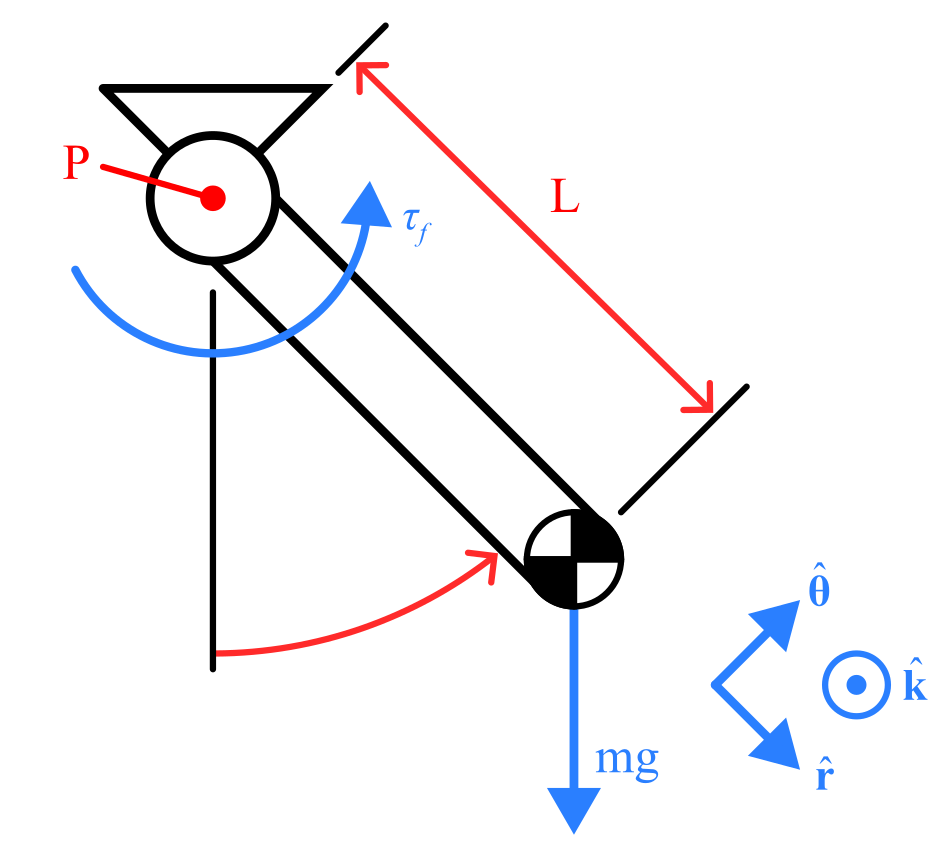
\includegraphics[width=0.3\linewidth,height=\textheight,keepaspectratio]{figures/PendulumDiagram.png}

}

\caption{\label{fig-pendulum-diagram}Coordinate system and torque
diagram for a simple pendulum.}

\end{figure}%

The moment of inertia of a point mass about the pivot is \(I_P = mL^2\),
so Newton's second law for rotation,
\(\left(\tau_P\right)_z = I_P \ddot{\theta}\), gives

\begin{equation}\protect\phantomsection\label{eq-eom-raw}{-mgL\sin\theta - b\dot{\theta} = mL^2 \ddot{\theta}.}\end{equation}

Rearranging into standard form yields a second-order nonlinear ODE:

\begin{equation}\protect\phantomsection\label{eq-eom}{\ddot{\theta} + 2\zeta\omega_n \dot{\theta} + \omega_n^2 \sin(\theta) = 0, \qquad \zeta = \frac{b}{2mL^2\omega_n}, \qquad \omega_n = \sqrt{\frac{g}{L}}}\end{equation}

where \(\omega_n\) is the natural frequency and \(\zeta\) is the damping
ratio. You can measure \(L\) directly with a ruler, but \(\zeta\)
depends on \(m\) and \(b\), which you will \emph{not} measure ---
instead, you will tune \(\zeta\) until the simulation matches your data.

\subsection{From Model to Simulation}\label{sec-model-to-sim}

Numerical ODE solvers (MATLAB's \texttt{ode45}, Python's
\texttt{solve\_ivp}) integrate systems of \emph{first-order} equations.
To simulate Equation~\ref{eq-eom}, we rewrite the single second-order
equation as two first-order equations by introducing the angular
velocity \(\omega = \dot\theta\) as a second state variable:

\begin{equation}\protect\phantomsection\label{eq-state-space}{\frac{d\theta}{dt} = \omega, \qquad \frac{d\omega}{dt} = -2\zeta\omega_n\omega - \omega_n^2\sin(\theta)}\end{equation}

The solver marches these equations forward in time from an initial
condition \(\left[\theta(0),\, \omega(0)\right]\) --- for your
experiment, the release angle and zero velocity. You will implement this
in Section~\ref{sec-part-6}.

\newpage{}

\section{Part-1: Set Up the ADS and WaveForms}\label{sec-part-1}

\subsection{Connect the ADS}\label{connect-the-ads}

\begin{enumerate}
\def\labelenumi{\arabic{enumi}.}
\tightlist
\item
  Ensure the Analog Discovery Studio is plugged into a wall outlet and
  powered on, then connect it to your computer via USB.
\item
  Open the \textbf{WaveForms} application. In the Device Manager, select
  \textbf{Analog Discovery Studio} and click \textbf{Select} (the same
  steps as Lab 01).
\item
  The WaveForms \textbf{Welcome} screen lists all available instruments;
  see Figure~\ref{fig-waveforms-welcome}. Identify the three you will
  use today:

  \begin{itemize}
  \tightlist
  \item
    \textbf{Supplies} --- controls the ADS power outputs
  \item
    \textbf{Scope} (oscilloscope) --- displays analog voltage vs.~time,
    live
  \item
    \textbf{Logger} --- records voltage over time and exports it to file
  \end{itemize}
\end{enumerate}

\begin{figure}

\centering{

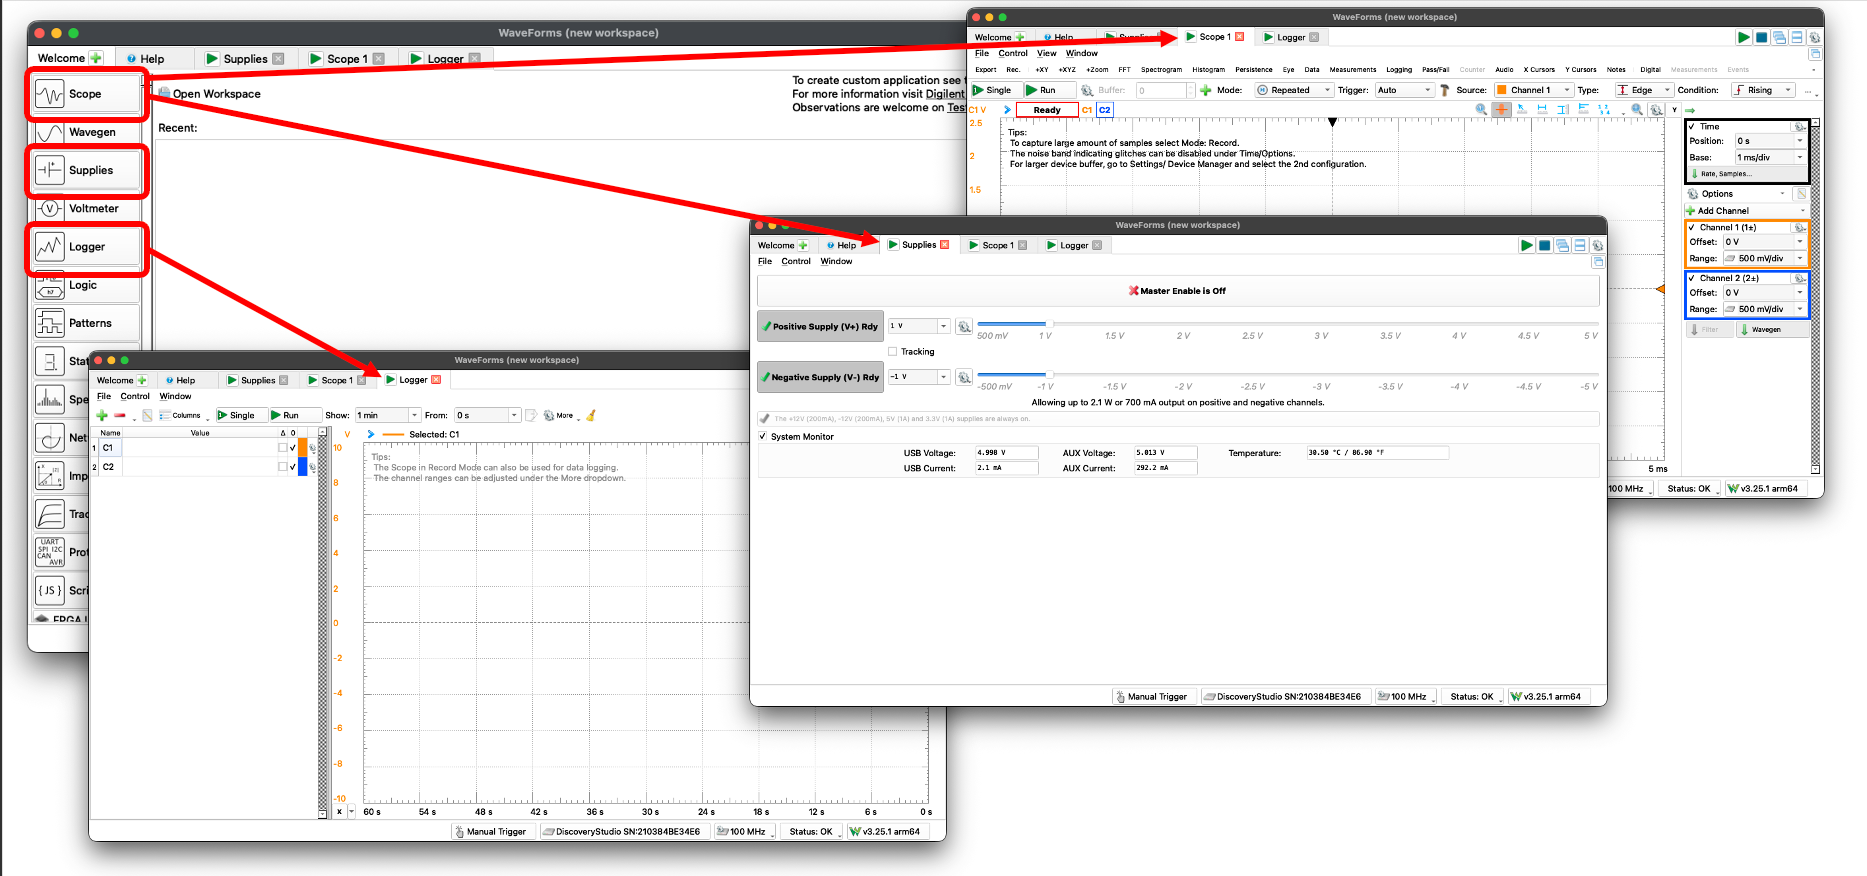
\includegraphics[width=1\linewidth,height=\textheight,keepaspectratio]{figures/Waveforms_Welcome.png}

}

\caption{\label{fig-waveforms-welcome}The WaveForms Welcome screen.
Annotations show the Supplies, Scope, and Logger instruments used in
this lab.}

\end{figure}%

\begin{tcolorbox}[enhanced jigsaw, arc=.35mm, bottomrule=.15mm, bottomtitle=1mm, breakable, colback=white, colbacktitle=quarto-callout-important-color!10!white, colframe=quarto-callout-important-color-frame, coltitle=black, left=2mm, leftrule=.75mm, opacityback=0, opacitybacktitle=0.6, rightrule=.15mm, title=\textcolor{quarto-callout-important-color}{\faExclamation}\hspace{0.5em}{Logbook Questions}, titlerule=0mm, toprule=.15mm, toptitle=1mm]

\textbf{Q1.} In your logbook, match each WaveForms instrument you'll use
today (Supplies, Scope, Logger) to a piece of traditional benchtop lab
equipment it replaces.

\end{tcolorbox}

\subsection{Enable the Power Supply}\label{enable-the-power-supply}

The potentiometer needs a stable reference voltage. You will use the
ADS's fixed \textbf{3.3 V} supply.

\begin{enumerate}
\def\labelenumi{\arabic{enumi}.}
\tightlist
\item
  Open \textbf{Supplies} in WaveForms.
\item
  Enable the \textbf{3.3 V} fixed supply and click \textbf{Master
  Enable}; see Figure~\ref{fig-supplies-setup}. Leave the ±12 V supplies
  off.
\item
  Verify the output with your DMM: measure between the \textbf{V+} pin
  and a \textbf{GND} pin on the ADS breadboard header.
\end{enumerate}

\begin{figure}

\centering{

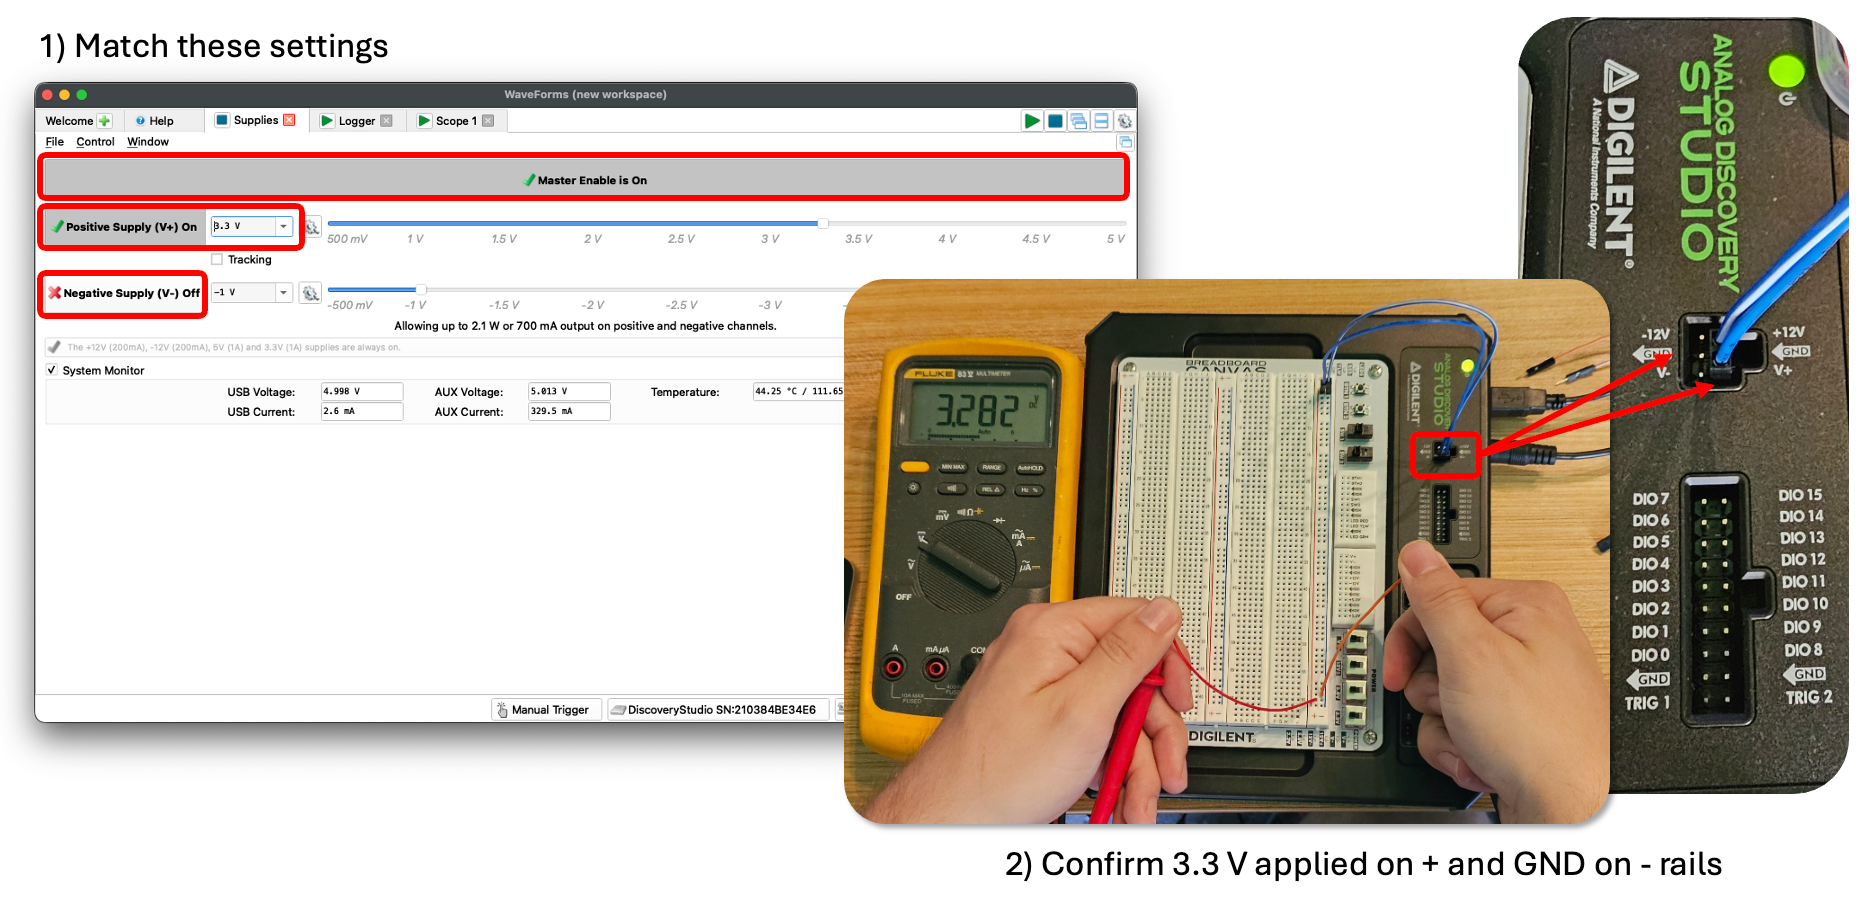
\includegraphics[width=1\linewidth,height=\textheight,keepaspectratio]{figures/Supplies_Setup.png}

}

\caption{\label{fig-supplies-setup}Supplies instrument with the 3.3 V
output enabled.}

\end{figure}%

\begin{tcolorbox}[enhanced jigsaw, arc=.35mm, bottomrule=.15mm, bottomtitle=1mm, breakable, colback=white, colbacktitle=quarto-callout-important-color!10!white, colframe=quarto-callout-important-color-frame, coltitle=black, left=2mm, leftrule=.75mm, opacityback=0, opacitybacktitle=0.6, rightrule=.15mm, title=\textcolor{quarto-callout-important-color}{\faExclamation}\hspace{0.5em}{Logbook Questions}, titlerule=0mm, toprule=.15mm, toptitle=1mm]

\textbf{Q2.} What voltage does your DMM read? Is it \emph{exactly} 3.3
V? Record the value. Why does it matter for your calibration whether
this supply drifts during the lab?

\end{tcolorbox}

\newpage{}

\section{Part-2: Build the Potentiometer Circuit}\label{sec-part-2}

Your main guide for this part is the annotated photo and circuit diagram
in Figure~\ref{fig-circuit-build} and Figure~\ref{fig-circuit-diagram}.
Study them first; the text below explains what you are looking at and
why each connection exists.

\begin{figure}

\centering{

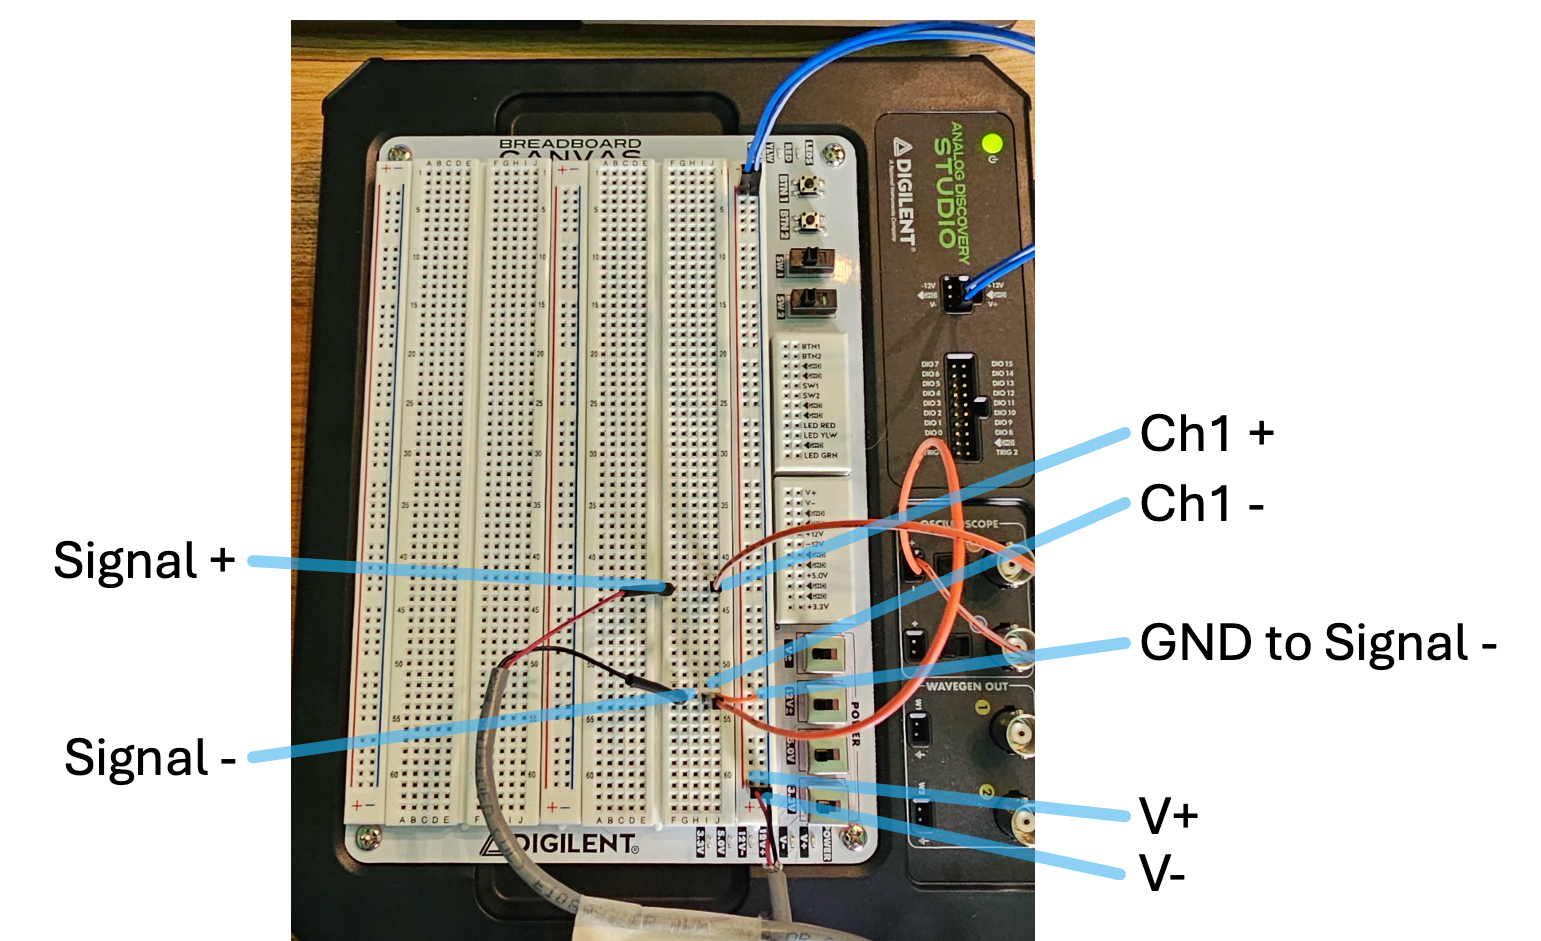
\includegraphics[width=1\linewidth,height=\textheight,keepaspectratio]{figures/Circuit_Build_ADS.png}

}

\caption{\label{fig-circuit-build}Annotated photo of the potentiometer
circuit built on the ADS breadboard.}

\end{figure}%

\begin{figure}

\centering{

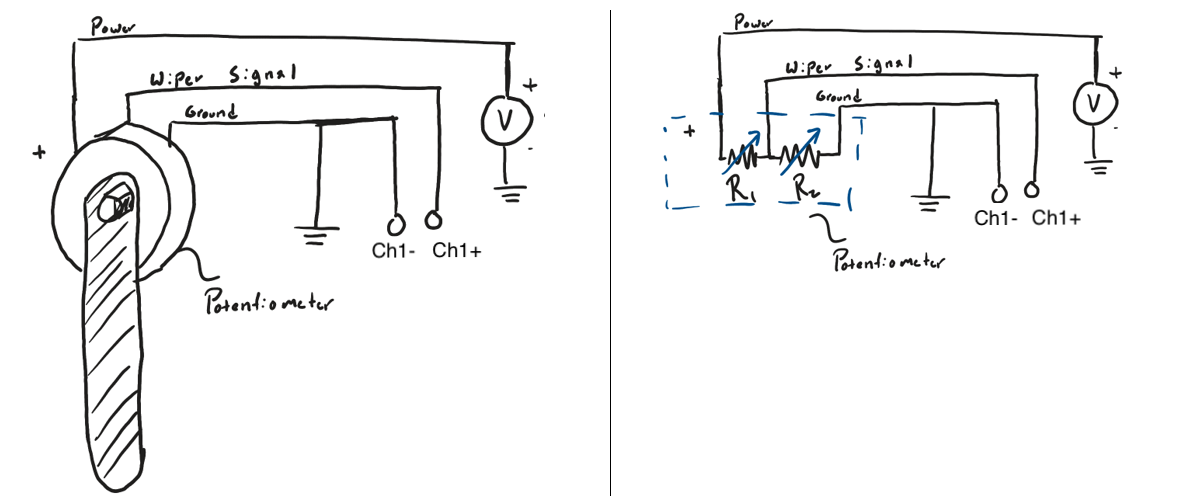
\includegraphics[width=1\linewidth,height=\textheight,keepaspectratio]{figures/Circuit_Diagram_Figs.png}

}

\caption{\label{fig-circuit-diagram}Potentiometer circuit diagram. The
wiper divides the total resistance into \(R_1\) and \(R_2\), which vary
with shaft angle, forming a voltage divider.}

\end{figure}%

The potentiometer has three leads, and the ADS analog inputs are
\textbf{differential} --- Channel 1 measures the voltage
\emph{difference} between its 1+ and 1− pins. That gives four
connections in total:

{\def\LTcaptype{none} % do not increment counter
\begin{longtable}[]{@{}
  >{\raggedright\arraybackslash}p{(\linewidth - 4\tabcolsep) * \real{0.4762}}
  >{\raggedright\arraybackslash}p{(\linewidth - 4\tabcolsep) * \real{0.3095}}
  >{\raggedright\arraybackslash}p{(\linewidth - 4\tabcolsep) * \real{0.2143}}@{}}
\toprule\noalign{}
\begin{minipage}[b]{\linewidth}\raggedright
Potentiometer lead
\end{minipage} & \begin{minipage}[b]{\linewidth}\raggedright
Connects to
\end{minipage} & \begin{minipage}[b]{\linewidth}\raggedright
Purpose
\end{minipage} \\
\midrule\noalign{}
\endhead
\bottomrule\noalign{}
\endlastfoot
End terminal (V+) & 3.3 V (V+) on ADS & Supplies the top of the
divider \\
End terminal (GND) & GND on ADS & Grounds the bottom of the divider \\
Wiper (center) & \textbf{1+} (Scope Ch. 1 positive) & The signal:
divider output voltage \\
--- (jumper) & GND rail → \textbf{1−} (Ch. 1 negative) & Gives the
differential input its reference \\
\end{longtable}
}

\begin{enumerate}
\def\labelenumi{\arabic{enumi}.}
\tightlist
\item
  Match your wiring to Figure~\ref{fig-circuit-build}, routing each
  connection through the breadboard rails as shown.
\item
  Before applying power, tug gently on each jumper to confirm it is
  seated, and check with your DMM (continuity mode) that V+ and GND are
  \textbf{not} shorted together.
\item
  Enable the supply, then slowly rotate the pendulum by hand while
  measuring the wiper voltage with your DMM. The voltage should vary
  smoothly across the swing range.
\end{enumerate}

\begin{tcolorbox}[enhanced jigsaw, arc=.35mm, bottomrule=.15mm, bottomtitle=1mm, breakable, colback=white, colbacktitle=quarto-callout-note-color!10!white, colframe=quarto-callout-note-color-frame, coltitle=black, left=2mm, leftrule=.75mm, opacityback=0, opacitybacktitle=0.6, rightrule=.15mm, title=\textcolor{quarto-callout-note-color}{\faInfo}\hspace{0.5em}{If the voltage jumps or drops suddenly}, titlerule=0mm, toprule=.15mm, toptitle=1mm]

The potentiometer body may be misaligned so that its dead zone (the
small angle where the wiper leaves the resistive track) falls inside the
swing range. Ask your TA --- they will loosen the grub screw, rotate the
potentiometer body until the jump occurs far outside the operating range
(near ±180°), and re-tighten it. Then re-test.

\end{tcolorbox}

\begin{tcolorbox}[enhanced jigsaw, arc=.35mm, bottomrule=.15mm, bottomtitle=1mm, breakable, colback=white, colbacktitle=quarto-callout-important-color!10!white, colframe=quarto-callout-important-color-frame, coltitle=black, left=2mm, leftrule=.75mm, opacityback=0, opacitybacktitle=0.6, rightrule=.15mm, title=\textcolor{quarto-callout-important-color}{\faExclamation}\hspace{0.5em}{Logbook Questions}, titlerule=0mm, toprule=.15mm, toptitle=1mm]

\textbf{Q3.} Sketch the schematic of your circuit in your logbook. Label
the supply, ground, wiper signal, and the ADS input pins.

\textbf{Q4.} Record the wiper voltages at the two extremes of the
pendulum's travel (about −90° and +90°). Roughly what fraction of the
0--3.3 V range does your sensor use?

\end{tcolorbox}

\newpage{}

\section{Part-3: Observe the Signal with the Scope}\label{sec-part-3}

Before recording anything, get to know your signal. Engineers
\emph{always} look at a live signal before trusting a logged file --- it
is the fastest way to catch a loose wire, a misaligned sensor, or a bad
setting.

\subsection{Configure the Scope}\label{configure-the-scope}

\begin{enumerate}
\def\labelenumi{\arabic{enumi}.}
\tightlist
\item
  Open \textbf{Scope} in WaveForms.
\item
  Ensure \textbf{Channel 1} is enabled.
\item
  Match the settings in Figure~\ref{fig-scope-setup}:

  \begin{itemize}
  \tightlist
  \item
    \textbf{Range:} 500 mV/div
  \item
    \textbf{Offset:} −1.65 V (centers the mid-travel voltage on screen)
  \item
    \textbf{Time base:} 200 ms/div
  \end{itemize}
\item
  Press \textbf{Run}. You should see the live voltage trace.
\end{enumerate}

\begin{figure}

\centering{

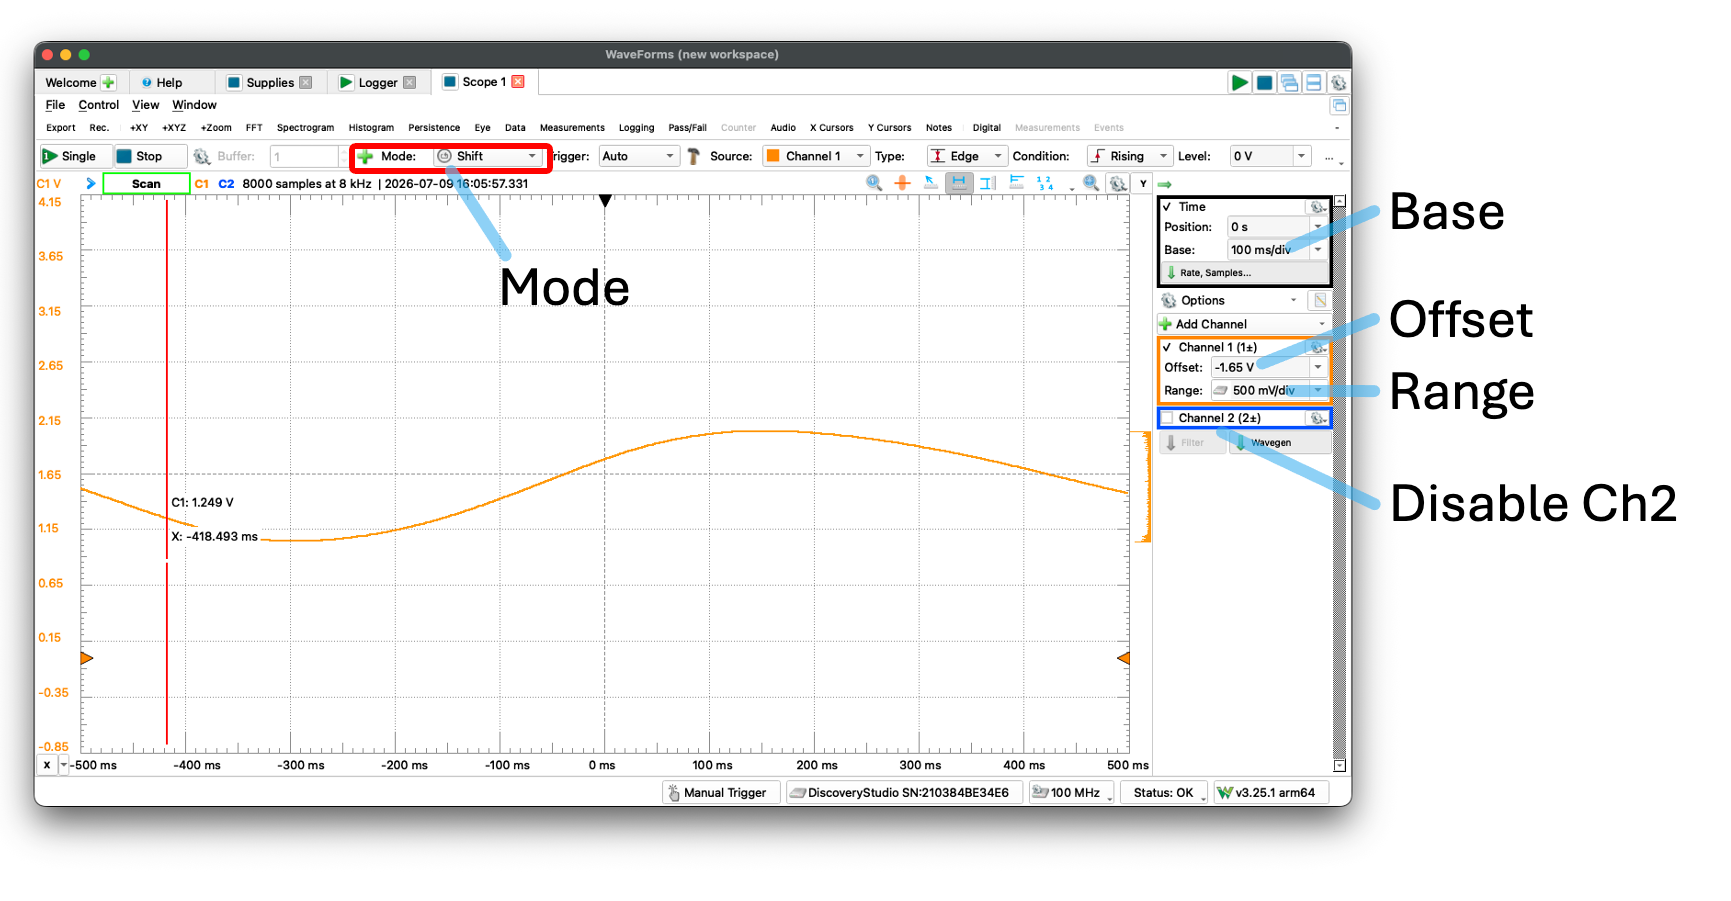
\includegraphics[width=1\linewidth,height=\textheight,keepaspectratio]{figures/Scope_Setup.png}

}

\caption{\label{fig-scope-setup}Scope configured to view the pendulum
signal. Annotations show channel enable, Range, Time base, and
Run/Stop.}

\end{figure}%

\subsection{Explore the Signal}\label{explore-the-signal}

\begin{enumerate}
\def\labelenumi{\arabic{enumi}.}
\setcounter{enumi}{4}
\tightlist
\item
  Slowly rotate the pendulum through its full range (about −90° to +90°)
  and watch the trace respond.
\item
  Lift the pendulum, release it, and let it swing freely. Watch the
  oscillation. Press \textbf{Stop} to freeze the display.
\item
  With the display frozen, open the \textbf{Cursors} panel and place two
  X (time) cursors one full oscillation apart; see
  Figure~\ref{fig-scope-cursors}. The readout shows the time difference
  --- a first estimate of the oscillation period.
\end{enumerate}

\begin{figure}

\centering{

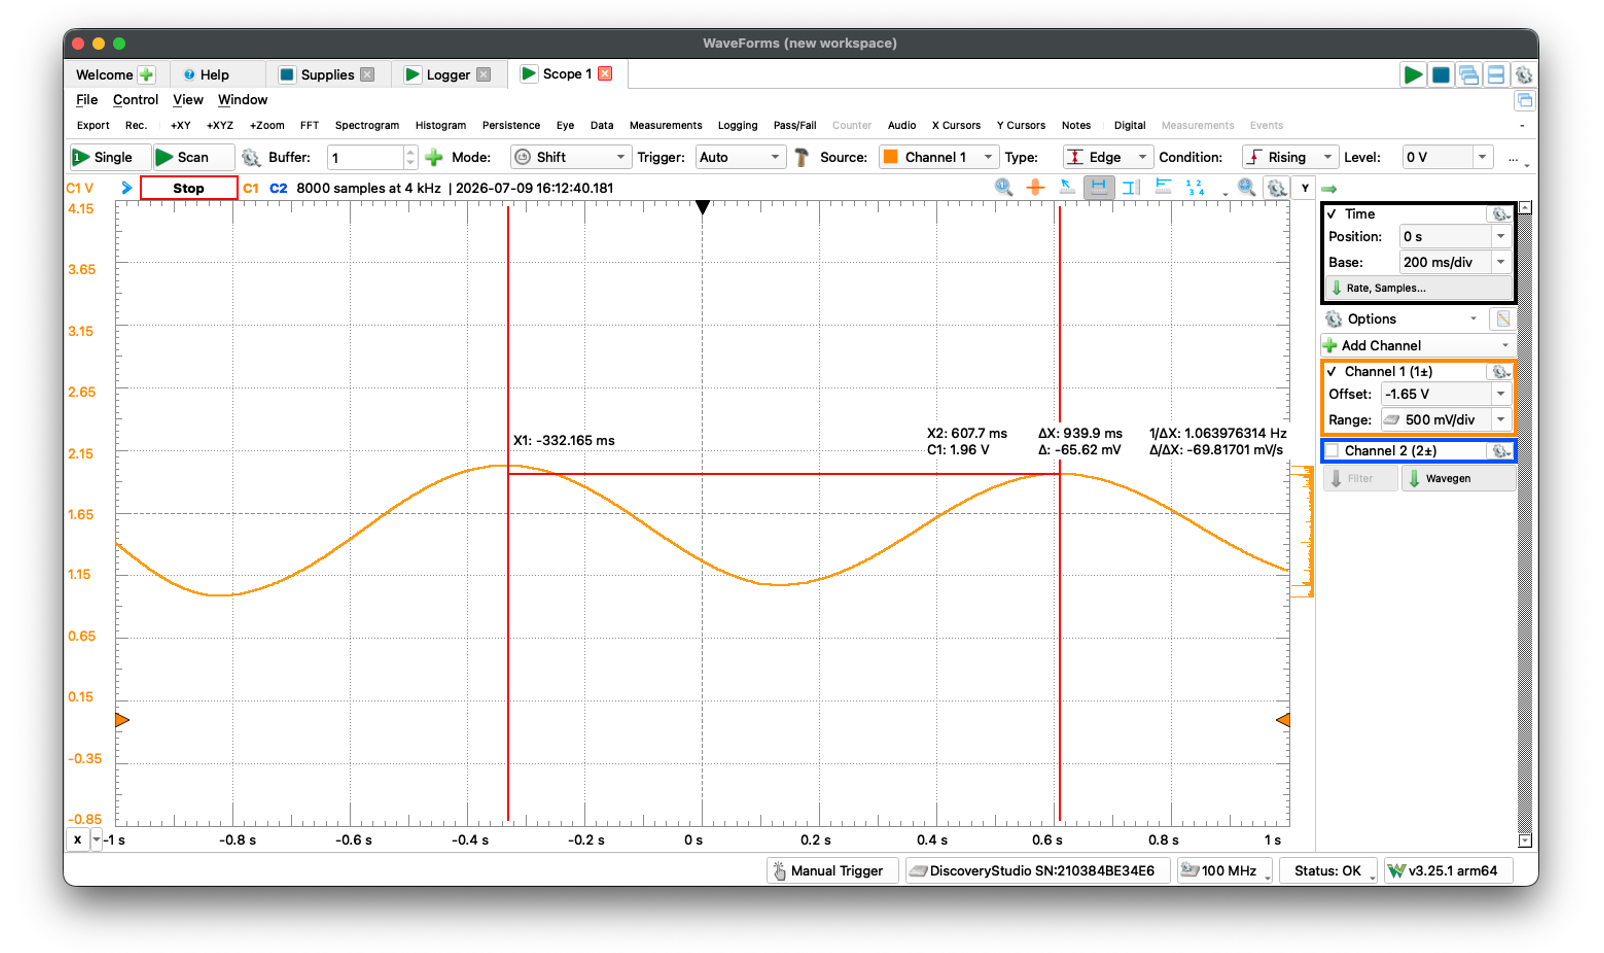
\includegraphics[width=1\linewidth,height=\textheight,keepaspectratio]{figures/Scope_Cursors.png}

}

\caption{\label{fig-scope-cursors}Using X cursors to measure the period
of one oscillation.}

\end{figure}%

\begin{tcolorbox}[enhanced jigsaw, arc=.35mm, bottomrule=.15mm, bottomtitle=1mm, breakable, colback=white, colbacktitle=quarto-callout-important-color!10!white, colframe=quarto-callout-important-color-frame, coltitle=black, left=2mm, leftrule=.75mm, opacityback=0, opacitybacktitle=0.6, rightrule=.15mm, title=\textcolor{quarto-callout-important-color}{\faExclamation}\hspace{0.5em}{Logbook Questions}, titlerule=0mm, toprule=.15mm, toptitle=1mm]

\textbf{Q5.} Sketch the frozen waveform in your logbook. Is it a sine
wave? Is the amplitude constant, or does it decay? Label your sketch
with the approximate period from the cursors.

\textbf{Q6.} Hold the pendulum still at 0° (straight down) and read the
mean voltage (Scope \textbf{Measurements} panel, or just the trace
level). How does it compare to what the voltage divider predicts for
mid-travel?

\end{tcolorbox}

\newpage{}

\section{Part-4: Calibrate the Sensor}\label{sec-part-4}

Here is the heart of the lab. A calibration converts sensor output
(volts) into the physical quantity you actually want (degrees). You will
hold the pendulum at a series of known angles, record a short voltage
dataset at each one, then fit Equation~\ref{eq-calibration} to the
results in Python.

\subsection{Set Up the Logger}\label{set-up-the-logger}

\begin{enumerate}
\def\labelenumi{\arabic{enumi}.}
\tightlist
\item
  Open \textbf{Logger} in WaveForms.
\item
  Configure Channel 1 to record the Scope Channel 1 voltage, and match
  the settings in Figure~\ref{fig-logger-setup}:

  \begin{itemize}
  \tightlist
  \item
    \textbf{Update:} 50 ms (i.e., 20 samples per second)
  \item
    \textbf{Duration:} 10 seconds
  \end{itemize}
\item
  You will export each recording as a CSV via \textbf{File → Export},
  using the same export settings as Lab 01; see
  Figure~\ref{fig-logger-export}.
\end{enumerate}

\begin{figure}

\centering{

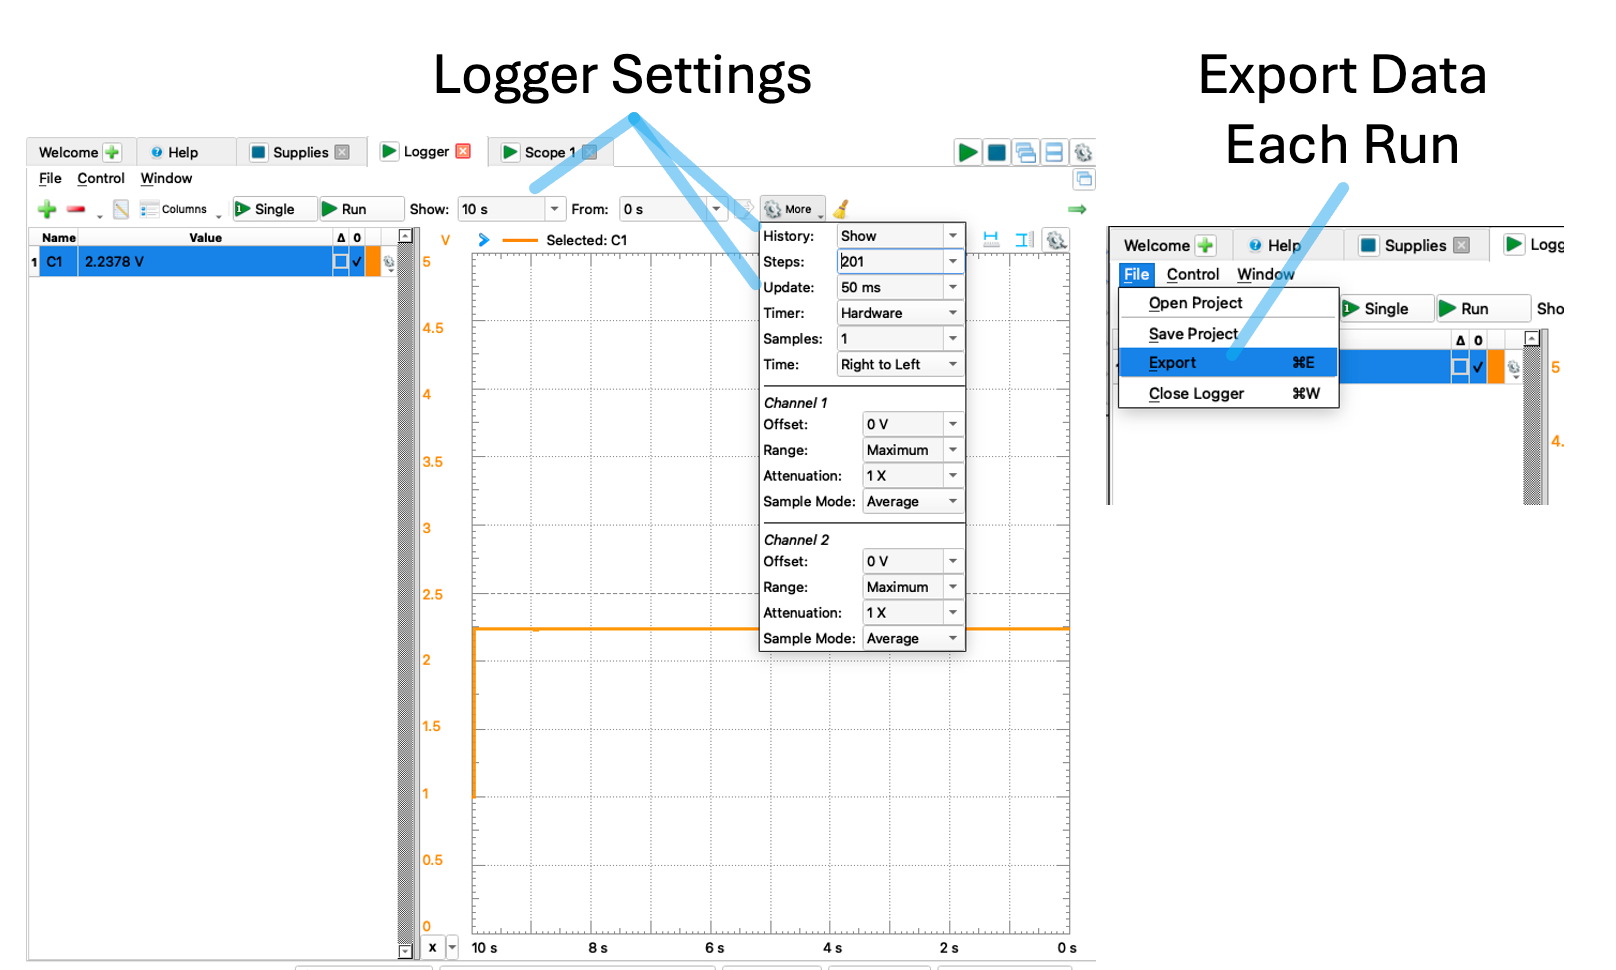
\includegraphics[width=1\linewidth,height=\textheight,keepaspectratio]{figures/Logger_Cal_Setup.png}

}

\caption{\label{fig-logger-setup}Logger configured for calibration
recordings (20 Hz, 10 s).}

\end{figure}%

\begin{figure}

\centering{

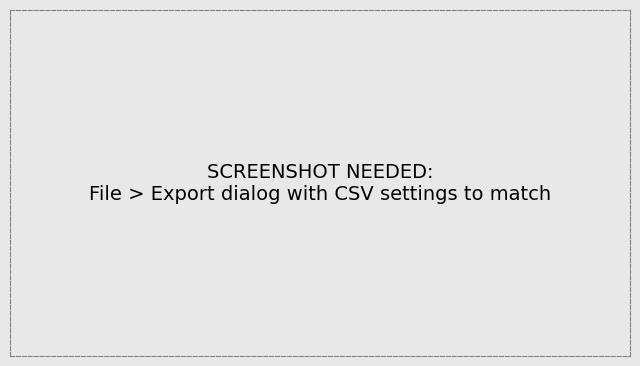
\includegraphics[width=0.7\linewidth,height=\textheight,keepaspectratio]{figures/Logger_Export.png}

}

\caption{\label{fig-logger-export}Exporting Logger data to CSV (match
these settings).}

\end{figure}%

\subsection{Collect Calibration Data}\label{collect-calibration-data}

Choose a reliable way to set the pendulum angle: the supplied
protractor, or a smartphone level app (e.g., \emph{Bubble Level}).
Angles follow the \textbf{right-hand rule} about the potentiometer
shaft, with \textbf{0° defined as the pendulum hanging straight down};
see Figure~\ref{fig-zero-position}.

\begin{figure}

\centering{

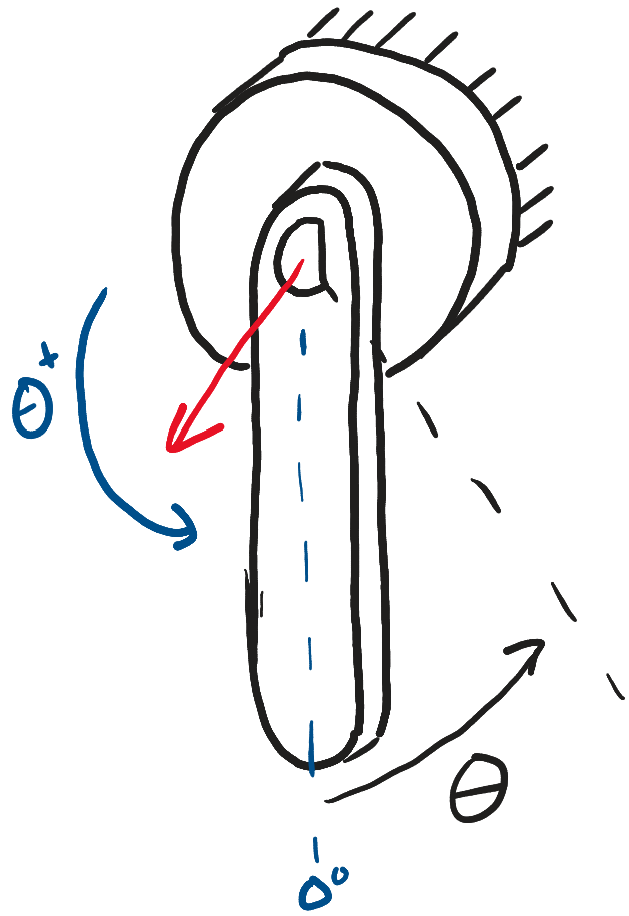
\includegraphics[width=0.25\linewidth,height=\textheight,keepaspectratio]{figures/Pendulum_Zero_Position_.png}

}

\caption{\label{fig-zero-position}Right-hand rule and pendulum zero
position.}

\end{figure}%

Record data at a \textbf{minimum of 11 angles} spanning the full range
--- for example:

−90°, −70°, −50°, −30°, −10°, 0°, 10°, 30°, 50°, 70°, 90°

For each angle:

\begin{enumerate}
\def\labelenumi{\arabic{enumi}.}
\tightlist
\item
  Hold the pendulum steady at the target angle (one partner holds, one
  runs the computer).
\item
  Run the Logger for the 10-second duration, then export the CSV to
  \texttt{ME3300/Lab\_02/Data/} using the naming convention
  \texttt{Ang\_p45Deg.csv} (positive angles) or \texttt{Ang\_n45Deg.csv}
  (negative) --- replace 45 with the actual angle, and always update the
  name \emph{before} exporting so you don't overwrite a previous run.
\item
  Log the angle in a table in your logbook like
  Table~\ref{tbl-calibration}. You will fill the voltage column from
  Python in the next step.
\end{enumerate}

\begin{longtable}[]{@{}cc@{}}
\caption{Example calibration logbook table (your voltages will differ
--- these are representative values for a 3.3 V
supply).}\label{tbl-calibration}\tabularnewline
\toprule\noalign{}
Pendulum Angle (Degrees) & Average Output Voltage (V) \\
\midrule\noalign{}
\endfirsthead
\toprule\noalign{}
Pendulum Angle (Degrees) & Average Output Voltage (V) \\
\midrule\noalign{}
\endhead
\bottomrule\noalign{}
\endlastfoot
−90° & 0.67 \\
−70° & 0.88 \\
−50° & 1.10 \\
−30° & 1.31 \\
−10° & 1.53 \\
0° & 1.65 \\
10° & 1.76 \\
30° & 1.98 \\
50° & 2.22 \\
70° & 2.44 \\
90° & 2.65 \\
\end{longtable}

\begin{tcolorbox}[enhanced jigsaw, arc=.35mm, bottomrule=.15mm, bottomtitle=1mm, breakable, colback=white, colbacktitle=quarto-callout-important-color!10!white, colframe=quarto-callout-important-color-frame, coltitle=black, left=2mm, leftrule=.75mm, opacityback=0, opacitybacktitle=0.6, rightrule=.15mm, title=\textcolor{quarto-callout-important-color}{\faExclamation}\hspace{0.5em}{Logbook Questions}, titlerule=0mm, toprule=.15mm, toptitle=1mm]

\textbf{Q7.} Before fitting anything: scan down your table. Does voltage
change by roughly the same amount for each 20° step? What does that
suggest about the linearity of your sensor?

\end{tcolorbox}

\subsection{Analyze the Calibration in
Python}\label{analyze-the-calibration-in-python}

Open your notebook \texttt{FirstName\_LastName\_Lab02.ipynb} in VS Code
(kernel: your \texttt{.venv}). As in Lab 01, a well-commented
\textbf{starter notebook} is available on Canvas, and the prelab
walkthrough covered every new syntax element used below.

\begin{tcolorbox}[enhanced jigsaw, arc=.35mm, bottomrule=.15mm, bottomtitle=1mm, breakable, colback=white, colbacktitle=quarto-callout-tip-color!10!white, colframe=quarto-callout-tip-color-frame, coltitle=black, left=2mm, leftrule=.75mm, opacityback=0, opacitybacktitle=0.6, rightrule=.15mm, title=\textcolor{quarto-callout-tip-color}{\faLightbulb}\hspace{0.5em}{Good notebook habits}, titlerule=0mm, toprule=.15mm, toptitle=1mm]

Structure your notebook with a markdown heading cell for each part of
the lab (\texttt{\#\#\ Part\ 4:\ Calibration}, etc.) and a sentence or
two describing what each code cell does and what you observed. Your
notebook is a lab record, not just code. Before submitting, always run
\textbf{Restart Kernel and Run All Cells} --- if it doesn't run
top-to-bottom cleanly, it isn't done.

\end{tcolorbox}

\textbf{Step 1 --- Load every calibration file and average it.}

In Lab 01 you loaded one CSV. Here you have 11 files that all need the
same treatment, which is exactly what a \textbf{\texttt{for} loop} is
for:

\begin{Shaded}
\begin{Highlighting}[]
\ImportTok{import}\NormalTok{ numpy }\ImportTok{as}\NormalTok{ np}
\ImportTok{import}\NormalTok{ matplotlib.pyplot }\ImportTok{as}\NormalTok{ plt}
\ImportTok{import}\NormalTok{ pandas }\ImportTok{as}\NormalTok{ pd}
\ImportTok{from}\NormalTok{ scipy }\ImportTok{import}\NormalTok{ stats}

\NormalTok{plt.rcParams[}\StringTok{\textquotesingle{}font.family\textquotesingle{}}\NormalTok{] }\OperatorTok{=} \StringTok{\textquotesingle{}serif\textquotesingle{}}
\NormalTok{plt.rcParams[}\StringTok{\textquotesingle{}font.serif\textquotesingle{}}\NormalTok{] }\OperatorTok{=}\NormalTok{ [}\StringTok{\textquotesingle{}Times New Roman\textquotesingle{}}\NormalTok{]}
\NormalTok{plt.rcParams[}\StringTok{\textquotesingle{}font.size\textquotesingle{}}\NormalTok{] }\OperatorTok{=} \DecValTok{10}

\CommentTok{\# The known angles you calibrated at — edit to match your actual angles}
\NormalTok{angles\_deg }\OperatorTok{=}\NormalTok{ np.array([}\OperatorTok{{-}}\DecValTok{90}\NormalTok{, }\OperatorTok{{-}}\DecValTok{70}\NormalTok{, }\OperatorTok{{-}}\DecValTok{50}\NormalTok{, }\OperatorTok{{-}}\DecValTok{30}\NormalTok{, }\OperatorTok{{-}}\DecValTok{10}\NormalTok{, }\DecValTok{0}\NormalTok{, }\DecValTok{10}\NormalTok{, }\DecValTok{30}\NormalTok{, }\DecValTok{50}\NormalTok{, }\DecValTok{70}\NormalTok{, }\DecValTok{90}\NormalTok{])}

\NormalTok{data\_dir }\OperatorTok{=} \StringTok{\textquotesingle{}../Data/\textquotesingle{}}
\NormalTok{mean\_voltages }\OperatorTok{=}\NormalTok{ np.zeros(}\BuiltInTok{len}\NormalTok{(angles\_deg))   }\CommentTok{\# empty array to fill in the loop}

\ControlFlowTok{for}\NormalTok{ i, angle }\KeywordTok{in} \BuiltInTok{enumerate}\NormalTok{(angles\_deg):}
\NormalTok{    sign }\OperatorTok{=} \StringTok{\textquotesingle{}n\textquotesingle{}} \ControlFlowTok{if}\NormalTok{ angle }\OperatorTok{\textless{}} \DecValTok{0} \ControlFlowTok{else} \StringTok{\textquotesingle{}p\textquotesingle{}}
\NormalTok{    filename }\OperatorTok{=} \SpecialStringTok{f\textquotesingle{}}\SpecialCharTok{\{}\NormalTok{data\_dir}\SpecialCharTok{\}}\SpecialStringTok{Ang\_}\SpecialCharTok{\{}\NormalTok{sign}\SpecialCharTok{\}\{}\BuiltInTok{abs}\NormalTok{(angle)}\SpecialCharTok{\}}\SpecialStringTok{Deg.csv\textquotesingle{}}
\NormalTok{    df }\OperatorTok{=}\NormalTok{ pd.read\_csv(filename, skiprows}\OperatorTok{=}\DecValTok{8}\NormalTok{)   }\CommentTok{\# skip WaveForms metadata lines}
\NormalTok{    mean\_voltages[i] }\OperatorTok{=}\NormalTok{ df.iloc[:, }\DecValTok{1}\NormalTok{].mean()  }\CommentTok{\# voltage is the 2nd column}

\BuiltInTok{print}\NormalTok{(mean\_voltages)   }\CommentTok{\# sanity check: should match your logbook table}
\end{Highlighting}
\end{Shaded}

New syntax to understand before you run this (all practiced in the
prelab):

\begin{itemize}
\tightlist
\item
  \textbf{\texttt{for\ i,\ angle\ in\ enumerate(angles\_deg):}} --- the
  loop body runs once per angle. \texttt{enumerate} hands you \emph{two}
  things each pass: the counter \texttt{i} (0, 1, 2, \ldots), used to
  store each result in the right slot of \texttt{mean\_voltages}, and
  the value \texttt{angle} itself, used to build the filename.
\item
  \textbf{\texttt{sign\ =\ \textquotesingle{}n\textquotesingle{}\ if\ angle\ \textless{}\ 0\ else\ \textquotesingle{}p\textquotesingle{}}}
  --- a one-line conditional: \texttt{sign} becomes
  \texttt{\textquotesingle{}n\textquotesingle{}} for negative angles and
  \texttt{\textquotesingle{}p\textquotesingle{}} otherwise, matching
  your file-naming convention.
\item
  \textbf{\texttt{f\textquotesingle{}\{data\_dir\}Ang\_\{sign\}\{abs(angle)\}Deg.csv\textquotesingle{}}}
  --- an \textbf{f-string}. Anything inside \texttt{\{\ \}} is replaced
  with the variable's value, so for \texttt{angle\ =\ -70} this produces
  \texttt{\textquotesingle{}../Data/Ang\_n70Deg.csv\textquotesingle{}}.
  F-strings are how you build filenames, labels, and annotations from
  variables.
\item
  \textbf{\texttt{df.iloc{[}:,\ 1{]}}} --- position-based DataFrame
  indexing: \emph{all rows} (\texttt{:}), \emph{second column}
  (\texttt{1} --- Python counts from 0). We use \texttt{.iloc} here
  because WaveForms may name columns differently depending on export
  settings, but the \emph{positions} (time first, voltage second) are
  consistent.
\end{itemize}

\begin{tcolorbox}[enhanced jigsaw, arc=.35mm, bottomrule=.15mm, bottomtitle=1mm, breakable, colback=white, colbacktitle=quarto-callout-warning-color!10!white, colframe=quarto-callout-warning-color-frame, coltitle=black, left=2mm, leftrule=.75mm, opacityback=0, opacitybacktitle=0.6, rightrule=.15mm, title=\textcolor{quarto-callout-warning-color}{\faExclamationTriangle}\hspace{0.5em}{Check \texttt{skiprows} against your actual file!}, titlerule=0mm, toprule=.15mm, toptitle=1mm]

WaveForms export files begin with several \texttt{\#} metadata lines
before the column headers and data. \textbf{Open one of your CSVs in VS
Code and count the lines to skip} --- do not assume the value in the
example is right for your export settings. If \texttt{pd.read\_csv}
gives strange results, this is the first thing to check. A quick
\texttt{df.head()} after loading shows you exactly what pandas thinks
the first rows are.

\end{tcolorbox}

\textbf{Step 2 --- Fit the calibration equation and quantify its
quality.}

You are fitting Equation~\ref{eq-calibration}, \(\theta = a_1 V + a_0\),
with \texttt{np.polyfit} exactly as in Lab 01 --- voltage is the input
\(x\), angle is the output \(y\). What's new is finishing the job:
reporting \emph{how good} the fit is. As in Lab 01, the 95\% confidence
interval on the fit is

\begin{equation}\protect\phantomsection\label{eq-confidence-level}{\theta_{cl} = \theta_{fit} \pm t_{\nu,95\%} \; s_{yx}}\end{equation}

where the \textbf{standard error of fit} is computed from the residuals
\(r_i = \theta_i - \theta_{c_i}\) (data minus fit):

\begin{equation}\protect\phantomsection\label{eq-standard-error-fit}{s_{yx} = \sqrt{\frac{\sum_{i=1}^{N} r_i^2}{\nu}} = \frac{\lVert r \rVert}{\sqrt{\nu}}, \qquad \nu = N - 2}\end{equation}

Note the second form: the \textbf{norm of the residuals},
\(\lVert r \rVert = \sqrt{\sum r_i^2}\), is just the numerator of
\(s_{yx}\) before dividing by the degrees of freedom. It is a single
number summarizing the total misfit, and \(s_{yx}\) is that misfit
converted to a per-point standard error. The \textbf{standard error of
the slope} is

\begin{equation}\protect\phantomsection\label{eq-slope-std-error}{S_{a_1} = s_{yx} \sqrt{\frac{1}{\sum_{i=1}^{N}\left(x_i - \bar{x}\right)^2}}}\end{equation}

where \(x\) here is voltage and \(\bar{x}\) its mean. \(S_{a_1}\)
carries the units of the slope (°/V) and tells you the uncertainty of
your calibration gain. The code implements these equations term by term:

\begin{Shaded}
\begin{Highlighting}[]
\CommentTok{\# {-}{-}{-} Fit: angle = a1 * voltage + a0  (Eq. 8) {-}{-}{-}}
\NormalTok{coeffs     }\OperatorTok{=}\NormalTok{ np.polyfit(mean\_voltages, angles\_deg, }\DecValTok{1}\NormalTok{)   }\CommentTok{\# [a1, a0]}
\NormalTok{angles\_fit }\OperatorTok{=}\NormalTok{ np.polyval(coeffs, mean\_voltages)}

\CommentTok{\# {-}{-}{-} Fit quality (Eqs. 9{-}11) {-}{-}{-}}
\NormalTok{N      }\OperatorTok{=} \BuiltInTok{len}\NormalTok{(angles\_deg)}
\NormalTok{nu     }\OperatorTok{=}\NormalTok{ N }\OperatorTok{{-}} \DecValTok{2}                                  \CommentTok{\# dof: 2 fit parameters}
\NormalTok{resid  }\OperatorTok{=}\NormalTok{ angles\_deg }\OperatorTok{{-}}\NormalTok{ angles\_fit                }\CommentTok{\# residuals r\_i}
\NormalTok{norm\_r }\OperatorTok{=}\NormalTok{ np.sqrt(np.}\BuiltInTok{sum}\NormalTok{(resid}\OperatorTok{**}\DecValTok{2}\NormalTok{))              }\CommentTok{\# norm of residuals ||r||}
\NormalTok{s\_yx   }\OperatorTok{=}\NormalTok{ norm\_r }\OperatorTok{/}\NormalTok{ np.sqrt(nu)                   }\CommentTok{\# standard error of fit}
\NormalTok{t\_val  }\OperatorTok{=}\NormalTok{ stats.t.ppf(}\FloatTok{0.975}\NormalTok{, df}\OperatorTok{=}\NormalTok{nu)              }\CommentTok{\# two{-}sided 95\% =\textgreater{} 0.975!}
\NormalTok{CI     }\OperatorTok{=}\NormalTok{ t\_val }\OperatorTok{*}\NormalTok{ s\_yx                           }\CommentTok{\# 95\% CI half{-}width}
\NormalTok{S\_a1   }\OperatorTok{=}\NormalTok{ s\_yx }\OperatorTok{/}\NormalTok{ np.sqrt(np.}\BuiltInTok{sum}\NormalTok{((mean\_voltages }\OperatorTok{{-}}\NormalTok{ np.mean(mean\_voltages))}\OperatorTok{**}\DecValTok{2}\NormalTok{))}

\BuiltInTok{print}\NormalTok{(}\SpecialStringTok{f"Calibration: theta = }\SpecialCharTok{\{}\NormalTok{coeffs[}\DecValTok{0}\NormalTok{]}\SpecialCharTok{:.4f\}}\SpecialStringTok{ V + }\SpecialCharTok{\{}\NormalTok{coeffs[}\DecValTok{1}\NormalTok{]}\SpecialCharTok{:.4f\}}\SpecialStringTok{"}\NormalTok{)}
\BuiltInTok{print}\NormalTok{(}\SpecialStringTok{f"norm = }\SpecialCharTok{\{}\NormalTok{norm\_r}\SpecialCharTok{:.4f\}}\SpecialStringTok{ deg, s\_yx = }\SpecialCharTok{\{}\NormalTok{s\_yx}\SpecialCharTok{:.4f\}}\SpecialStringTok{ deg, S\_a1 = }\SpecialCharTok{\{}\NormalTok{S\_a1}\SpecialCharTok{:.4f\}}\SpecialStringTok{ deg/V"}\NormalTok{)}

\CommentTok{\# Save the coefficients — you will reuse this calibration in later labs}
\NormalTok{np.savetxt(}\StringTok{\textquotesingle{}../Data/calibration\_coeffs.csv\textquotesingle{}}\NormalTok{, coeffs,}
\NormalTok{           header}\OperatorTok{=}\StringTok{\textquotesingle{}a1 (deg/V), a0 (deg)\textquotesingle{}}\NormalTok{, delimiter}\OperatorTok{=}\StringTok{\textquotesingle{},\textquotesingle{}}\NormalTok{)}
\end{Highlighting}
\end{Shaded}

Recall from Lab 01: \texttt{stats.t.ppf()} takes a \emph{one-tailed}
cumulative probability, so a two-sided 95\% interval requires
\(1 - 0.05/2 = 0.975\). Check yourself against your t-table: for
\(\nu = 9\), \(t_{9,95\%} = 2.262\).

\textbf{Step 3 --- Make the calibration plot.}

Nothing here is new --- this is Lab 01 plotting with your new results.
Build the figure to match Figure~\ref{fig-example-calibration}, using
the format requirements in the Post-Lab section. Annotate it (using
\texttt{ax.text} and an f-string) with the calibration equation, the
norm of residuals, \(s_{yx}\), and \(S_{a_1}\), each with 4 decimal
places and units. Save \textbf{.pdf} and \textbf{.png} copies at 600 DPI
to your \texttt{Figures} folder.

\begin{tcolorbox}[enhanced jigsaw, arc=.35mm, bottomrule=.15mm, bottomtitle=1mm, breakable, colback=white, colbacktitle=quarto-callout-important-color!10!white, colframe=quarto-callout-important-color-frame, coltitle=black, left=2mm, leftrule=.75mm, opacityback=0, opacitybacktitle=0.6, rightrule=.15mm, title=\textcolor{quarto-callout-important-color}{\faExclamation}\hspace{0.5em}{Logbook Questions}, titlerule=0mm, toprule=.15mm, toptitle=1mm]

\textbf{Q8.} Write your calibration equation in your logbook with units
on both coefficients.

\textbf{Q9.} In one or two sentences: what do the norm of residuals and
\(s_{yx}\) tell you about the quality of your fit? What would a much
larger \(s_{yx}\) mean physically for angle measurements made with this
sensor?

\end{tcolorbox}

\subsection{Example Result}\label{example-result}

\begin{figure}

\centering{

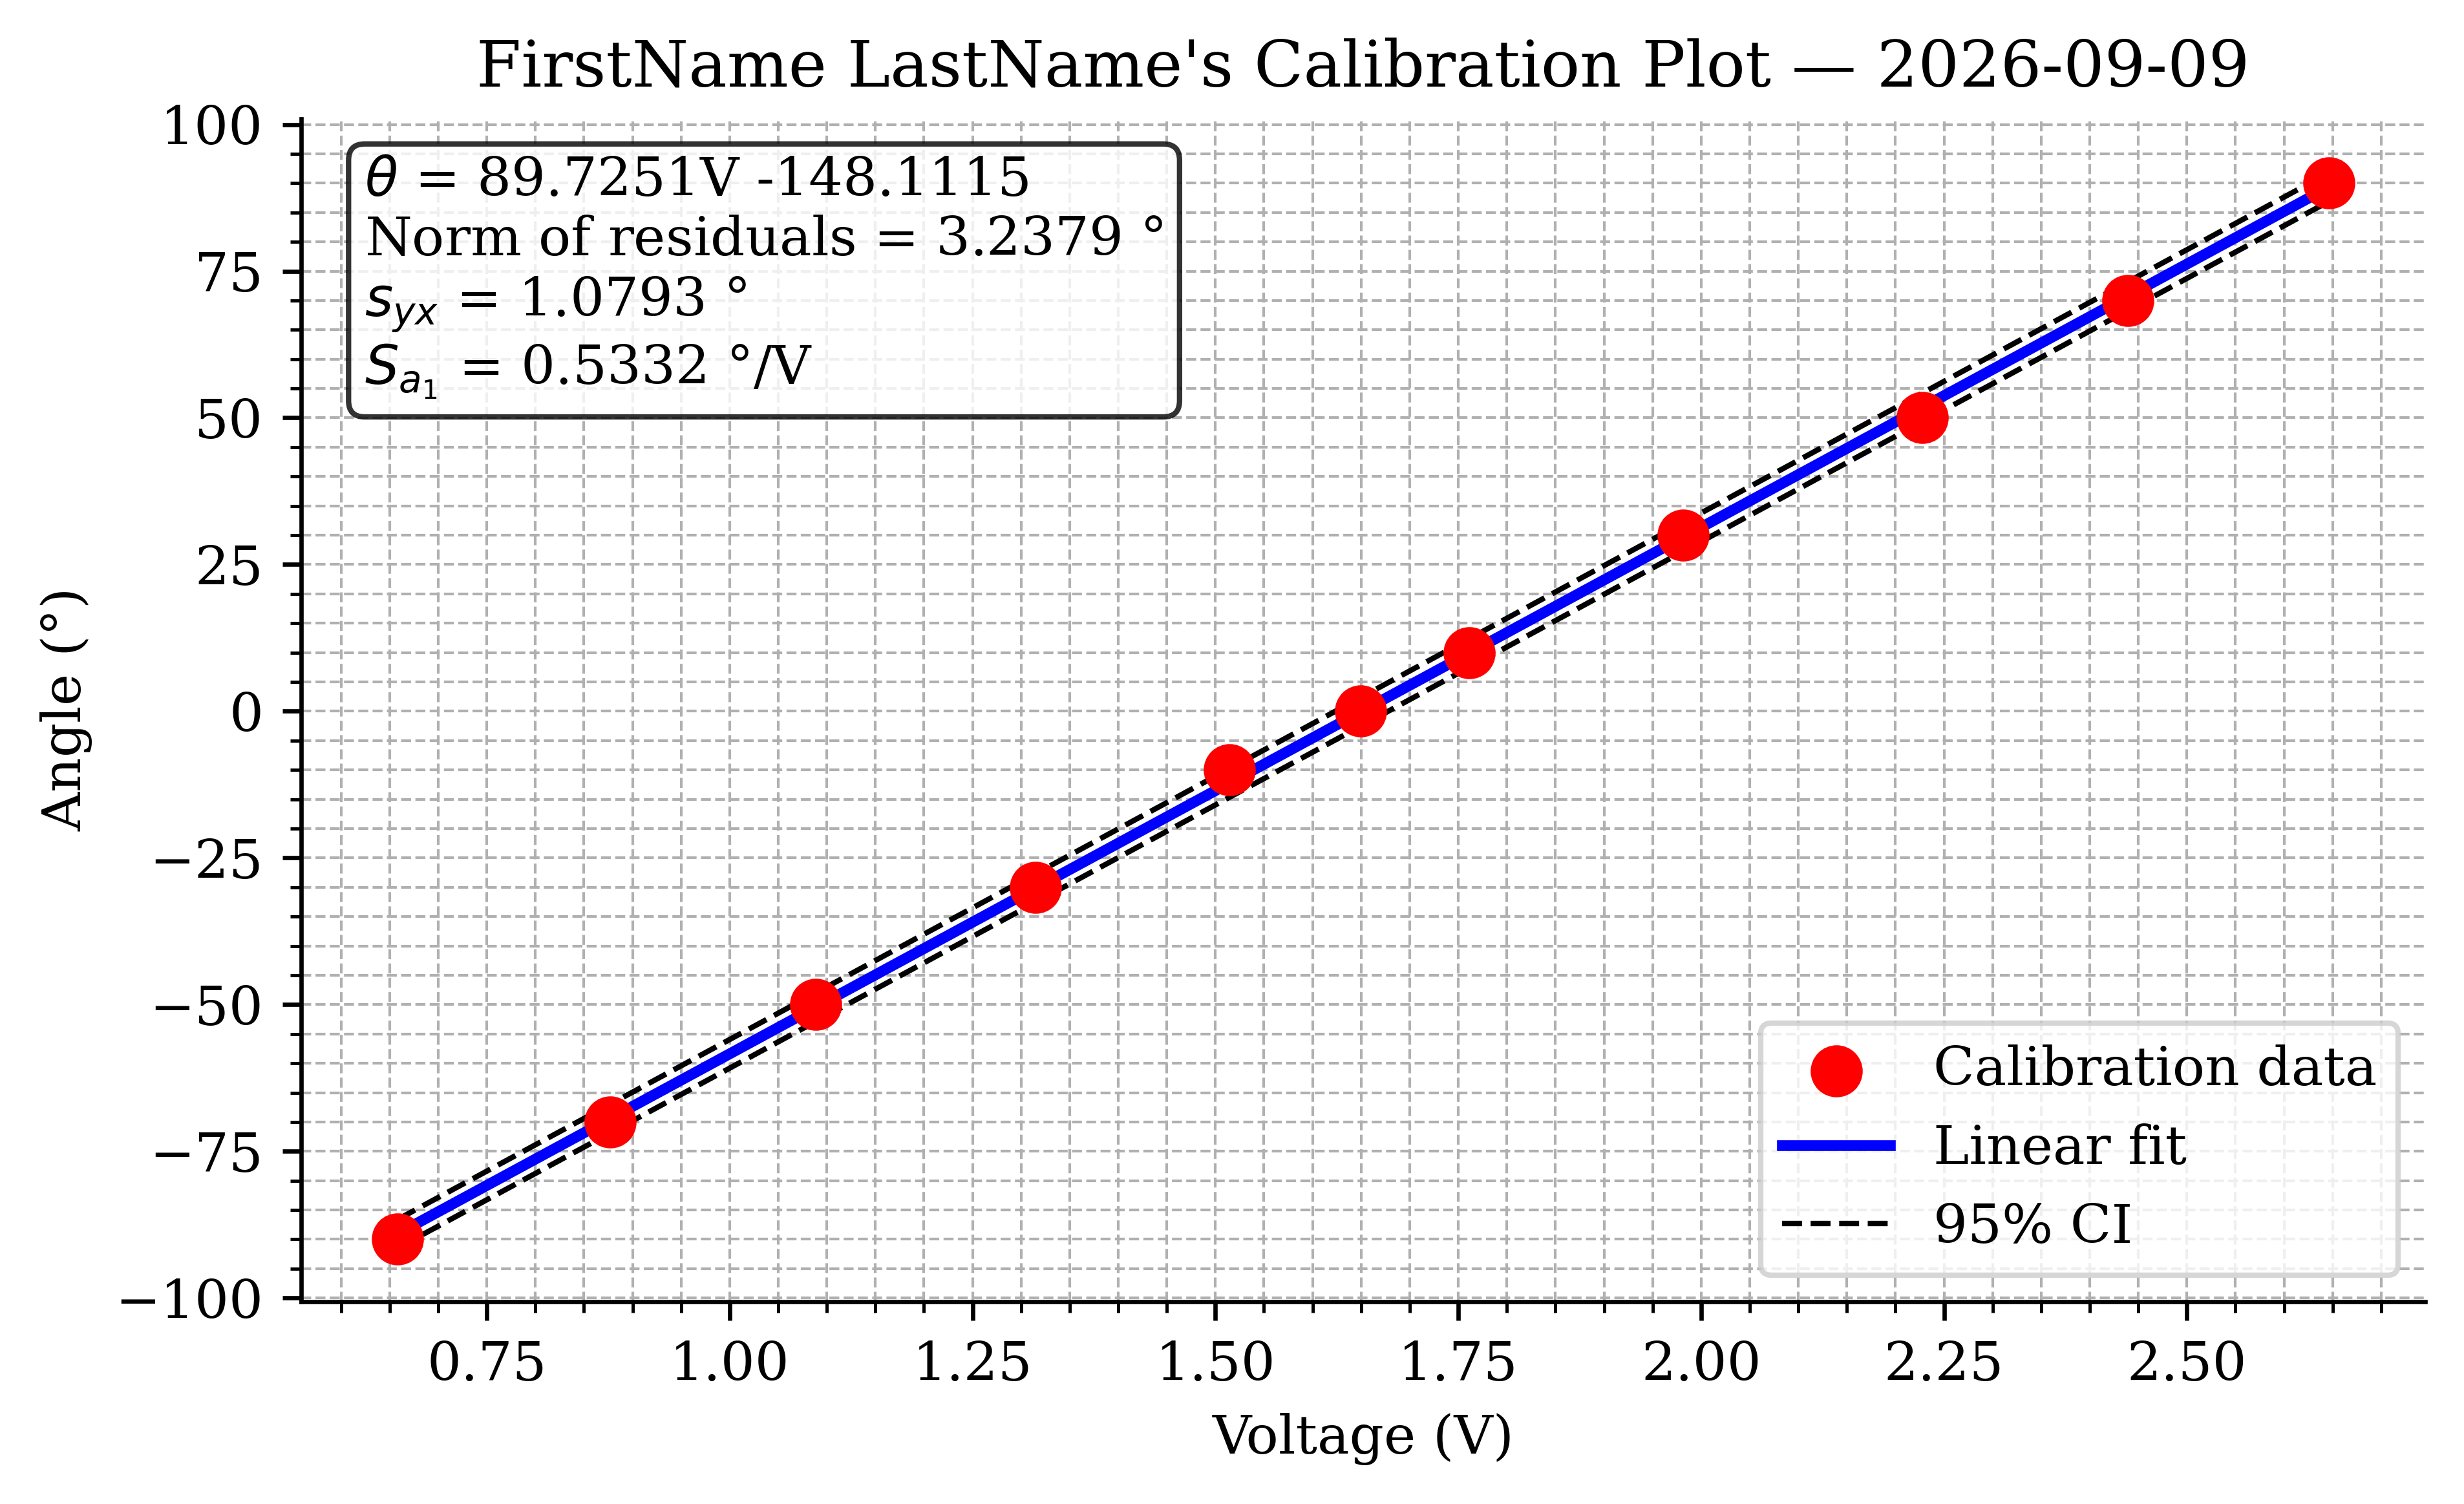
\includegraphics[width=6.5in,height=\textheight,keepaspectratio]{figures/Python/FirstName_LastName_Lab02_Calibration.png}

}

\caption{\label{fig-example-calibration}Example calibration plot
(made-up data). Your values will differ, but your formatting and
annotations should match.}

\end{figure}%

\newpage{}

\section{Part-5: Record and Analyze a Free Swing}\label{sec-part-5}

With a trusted calibration in hand, you can now make a real dynamic
measurement.

\subsection{Record the Swing}\label{record-the-swing}

\begin{enumerate}
\def\labelenumi{\arabic{enumi}.}
\tightlist
\item
  In the \textbf{Logger}, change the settings for a faster, longer
  recording:

  \begin{itemize}
  \tightlist
  \item
    \textbf{Update:} 10 ms (100 samples per second --- fast enough to
    resolve a \textasciitilde1 s oscillation smoothly)
  \item
    \textbf{Duration:} 20 seconds
  \end{itemize}
\item
  One partner holds the pendulum at approximately \textbf{+90°}
  (horizontal); the other starts the recording.
\item
  A second or two after the recording starts, \textbf{release the
  pendulum smoothly} --- let go, don't push.
\item
  Let it swing until the recording ends, then export the CSV as
  \texttt{FirstName\_LastName\_Lab02\_Swing.csv} to
  \texttt{ME3300/Lab\_02/Data/}.
\item
  Open the file in VS Code and confirm it contains what you expect
  before moving on.
\end{enumerate}

\subsection{Load, Calibrate, and Trim the
Data}\label{load-calibrate-and-trim-the-data}

Back in your notebook, load the swing recording, convert voltage to
angle with your calibration, and trim the recording so \(t = 0\) is the
moment of release:

\begin{Shaded}
\begin{Highlighting}[]
\CommentTok{\# Load swing data (check skiprows against your file, as before)}
\NormalTok{swing    }\OperatorTok{=}\NormalTok{ pd.read\_csv(}\StringTok{\textquotesingle{}../Data/FirstName\_LastName\_Lab02\_Swing.csv\textquotesingle{}}\NormalTok{, skiprows}\OperatorTok{=}\DecValTok{8}\NormalTok{)}
\NormalTok{time\_raw }\OperatorTok{=}\NormalTok{ swing.iloc[:, }\DecValTok{0}\NormalTok{].values     }\CommentTok{\# 1st column: time (s)}
\NormalTok{volt\_raw }\OperatorTok{=}\NormalTok{ swing.iloc[:, }\DecValTok{1}\NormalTok{].values     }\CommentTok{\# 2nd column: voltage (V)}

\CommentTok{\# Apply your calibration equation (Eq. 2): volts {-}\textgreater{} degrees}
\NormalTok{angle\_raw }\OperatorTok{=}\NormalTok{ np.polyval(coeffs, volt\_raw)}

\CommentTok{\# Trim so t = 0 is the release: find the first significant change in voltage}
\NormalTok{dv    }\OperatorTok{=}\NormalTok{ np.}\BuiltInTok{abs}\NormalTok{(np.diff(volt\_raw))      }\CommentTok{\# change between adjacent samples}
\NormalTok{idx0  }\OperatorTok{=}\NormalTok{ np.argmax(dv }\OperatorTok{\textgreater{}} \FloatTok{0.01}\NormalTok{)           }\CommentTok{\# index of FIRST sample where dv \textgreater{} 0.01 V}
\NormalTok{time  }\OperatorTok{=}\NormalTok{ time\_raw[idx0:] }\OperatorTok{{-}}\NormalTok{ time\_raw[idx0]}
\NormalTok{angle }\OperatorTok{=}\NormalTok{ angle\_raw[idx0:]}
\end{Highlighting}
\end{Shaded}

Two new tools here, both practiced in the prelab:

\begin{itemize}
\tightlist
\item
  \textbf{\texttt{np.diff(volt\_raw)}} returns the difference between
  each pair of adjacent samples --- effectively how fast the signal is
  changing, sample to sample. While the pendulum is held still, these
  differences are tiny (just noise); at release they jump.
\item
  \textbf{\texttt{np.argmax(dv\ \textgreater{}\ 0.01)}} --- the
  comparison \texttt{dv\ \textgreater{}\ 0.01} produces an array of
  \texttt{True}/\texttt{False} values, and \texttt{argmax} returns the
  index of the first \texttt{True} (since \texttt{True} counts as 1).
  Together they locate the first sample where the signal changed by more
  than 10 mV: the release. The \texttt{{[}idx0:{]}} slice then discards
  everything before that moment, and subtracting
  \texttt{time\_raw{[}idx0{]}} restarts the clock at zero.
\end{itemize}

\begin{tcolorbox}[enhanced jigsaw, arc=.35mm, bottomrule=.15mm, bottomtitle=1mm, breakable, colback=white, colbacktitle=quarto-callout-tip-color!10!white, colframe=quarto-callout-tip-color-frame, coltitle=black, left=2mm, leftrule=.75mm, opacityback=0, opacitybacktitle=0.6, rightrule=.15mm, title=\textcolor{quarto-callout-tip-color}{\faLightbulb}\hspace{0.5em}{Debug it yourself}, titlerule=0mm, toprule=.15mm, toptitle=1mm]

If your trim grabs the wrong moment, don't guess --- \emph{look}. Plot
\texttt{volt\_raw} against \texttt{time\_raw} (a two-line throwaway plot
is fine) and see where the release actually happens; then plot
\texttt{dv} and see whether 0.01 V is a sensible threshold for
\emph{your} noise level. Making quick diagnostic plots is the single
most useful debugging habit in experimental work --- most ``code bugs''
in this course are actually data surprises you'd spot instantly on a
plot.

\end{tcolorbox}

\subsection{Plot the Swing and Measure the
Period}\label{plot-the-swing-and-measure-the-period}

Plot \texttt{angle} vs.~\texttt{time} as a solid red line (2 pt) with
Lab 01 formatting --- this figure will become your final swing plot once
you overlay the model in Section~\ref{sec-part-6}, so build it carefully
now. From the plot, determine:

\begin{itemize}
\tightlist
\item
  the \textbf{damped period} \(T_d\): the time of one full oscillation.
  For better accuracy, measure the time across several periods (e.g., 5)
  and divide.
\item
  the \textbf{damped frequency} \(\omega_d = 2\pi / T_d\) in rad/s.
\end{itemize}

\begin{tcolorbox}[enhanced jigsaw, arc=.35mm, bottomrule=.15mm, bottomtitle=1mm, breakable, colback=white, colbacktitle=quarto-callout-important-color!10!white, colframe=quarto-callout-important-color-frame, coltitle=black, left=2mm, leftrule=.75mm, opacityback=0, opacitybacktitle=0.6, rightrule=.15mm, title=\textcolor{quarto-callout-important-color}{\faExclamation}\hspace{0.5em}{Logbook Questions}, titlerule=0mm, toprule=.15mm, toptitle=1mm]

\textbf{Q10.} Record \(T_d\) and \(\omega_d\) in your logbook. How does
\(T_d\) compare to the cursor estimate you made on the Scope in Part 3?

\textbf{Q11.} Does the oscillation period visibly change as the
amplitude decays? Look closely at early vs.~late cycles. (Keep
Equation~\ref{eq-eom} in mind: is this system exactly linear?)

\end{tcolorbox}

\newpage{}

\section{Part-6: Simulate the Model and Match It to Your
Data}\label{sec-part-6}

Now for the payoff: does the simple pendulum model of
Section~\ref{sec-pendulum-model} actually describe your pendulum? You
will simulate Equation~\ref{eq-eom} with
\texttt{scipy.integrate.solve\_ivp} (Python's counterpart to MATLAB's
\texttt{ode45}) and tune the model until it overlays your measurement.

\subsection{Implement the Simulation}\label{implement-the-simulation}

As explained in Section~\ref{sec-model-to-sim}, the solver needs the
second-order model rewritten as the two first-order equations of
Equation~\ref{eq-state-space}. In code, that pair of equations becomes a
small \textbf{function} that the solver calls over and over:

\begin{Shaded}
\begin{Highlighting}[]
\ImportTok{from}\NormalTok{ scipy.integrate }\ImportTok{import}\NormalTok{ solve\_ivp}

\CommentTok{\# {-}{-}{-} Model parameters {-}{-}{-}}
\NormalTok{L   }\OperatorTok{=} \FloatTok{0.30}                  \CommentTok{\# pendulum length (m) — MEASURE yours with a ruler}
\NormalTok{g   }\OperatorTok{=} \FloatTok{9.81}                  \CommentTok{\# gravitational acceleration (m/s\^{}2)}
\NormalTok{omega\_n }\OperatorTok{=}\NormalTok{ np.sqrt(g }\OperatorTok{/}\NormalTok{ L)    }\CommentTok{\# natural frequency (rad/s), Eq. 6}

\NormalTok{zeta }\OperatorTok{=} \FloatTok{0.05}                 \CommentTok{\# damping ratio — initial guess, you will tune this}

\CommentTok{\# {-}{-}{-} Initial conditions {-}{-}{-}}
\NormalTok{theta0 }\OperatorTok{=}\NormalTok{ np.radians(}\FloatTok{90.0}\NormalTok{)   }\CommentTok{\# release angle (rad) — match your actual release}
\NormalTok{omega0 }\OperatorTok{=} \FloatTok{0.0}                \CommentTok{\# released from rest}

\KeywordTok{def}\NormalTok{ pendulum\_ode(t, y):}
    \CommentTok{"""State derivative for the damped simple pendulum (Eq. 7)."""}
\NormalTok{    theta, omega }\OperatorTok{=}\NormalTok{ y                       }\CommentTok{\# unpack the state vector}
\NormalTok{    dtheta\_dt }\OperatorTok{=}\NormalTok{ omega}
\NormalTok{    domega\_dt }\OperatorTok{=} \OperatorTok{{-}}\DecValTok{2}\OperatorTok{*}\NormalTok{zeta}\OperatorTok{*}\NormalTok{omega\_n}\OperatorTok{*}\NormalTok{omega }\OperatorTok{{-}}\NormalTok{ omega\_n}\OperatorTok{**}\DecValTok{2} \OperatorTok{*}\NormalTok{ np.sin(theta)}
    \ControlFlowTok{return}\NormalTok{ [dtheta\_dt, domega\_dt]}

\CommentTok{\# {-}{-}{-} Solve over the same time range as the experiment {-}{-}{-}}
\NormalTok{t\_eval }\OperatorTok{=}\NormalTok{ np.linspace(time[}\DecValTok{0}\NormalTok{], time[}\OperatorTok{{-}}\DecValTok{1}\NormalTok{], }\DecValTok{2000}\NormalTok{)}
\NormalTok{sol }\OperatorTok{=}\NormalTok{ solve\_ivp(pendulum\_ode, (time[}\DecValTok{0}\NormalTok{], time[}\OperatorTok{{-}}\DecValTok{1}\NormalTok{]), [theta0, omega0],}
\NormalTok{                t\_eval}\OperatorTok{=}\NormalTok{t\_eval, max\_step}\OperatorTok{=}\FloatTok{0.005}\NormalTok{)}

\NormalTok{theta\_model\_deg }\OperatorTok{=}\NormalTok{ np.degrees(sol.y[}\DecValTok{0}\NormalTok{])}
\end{Highlighting}
\end{Shaded}

Walk through what each piece does:

\begin{itemize}
\tightlist
\item
  \textbf{\texttt{def\ pendulum\_ode(t,\ y):}} defines your own function
  --- the first time you've written one in this course. The solver hands
  it the current time \texttt{t} and current state \texttt{y}
  \(= [\theta, \omega]\), and the function must \texttt{return} the
  state's derivatives \([\dot\theta, \dot\omega]\). Compare the two
  \texttt{d...\_dt} lines to Equation~\ref{eq-state-space} --- they are
  a direct transcription.
\item
  \textbf{\texttt{theta,\ omega\ =\ y}} unpacks the two-element state
  vector into named variables so the physics reads clearly.
\item
  \textbf{\texttt{solve\_ivp(fun,\ t\_span,\ y0,\ ...)}} takes the
  derivative function, the time interval \texttt{(start,\ stop)}, and
  the initial state \texttt{{[}theta0,\ omega0{]}}, and numerically
  integrates forward --- just like \texttt{ode45(@fun,\ tspan,\ y0)} in
  MATLAB. By default it uses the same Runge--Kutta 4(5) algorithm.
\item
  \textbf{\texttt{t\_eval}} tells the solver where to report the
  solution (a dense grid gives a smooth plotted curve), and
  \textbf{\texttt{max\_step=0.005}} caps the internal step size so the
  solver can't step over the fast oscillations.
\item
  The solution comes back in \texttt{sol}: \texttt{sol.t} holds the
  times, and \texttt{sol.y{[}0{]}} holds the first state variable
  (\(\theta\), in radians) --- hence \texttt{np.degrees(...)} for
  plotting alongside your data.
\end{itemize}

\subsection{Overlay and Tune}\label{overlay-and-tune}

Add the model to your swing plot as a dashed blue line (2 pt),
re-render, and compare. Then iterate --- change one parameter at a time
and re-run:

\begin{enumerate}
\def\labelenumi{\arabic{enumi}.}
\tightlist
\item
  \textbf{Period wrong?} Adjust \texttt{L}. The model period is set by
  \(\omega_n = \sqrt{g/L}\), so if the model oscillates too fast, your
  effective length is longer than you measured (remember: the model
  wants the distance to the \emph{center of mass}, not to the tip).
\item
  \textbf{Decay rate wrong?} Adjust \texttt{zeta}. Larger \(\zeta\)
  makes the model amplitude die out faster.
\item
  \textbf{First swing misaligned?} Adjust \texttt{theta0} --- your
  actual release angle may not have been exactly 90°.
\end{enumerate}

Aim for close agreement over the first several oscillations; do not
expect perfection. It is normal --- and physically informative --- for
the model and data to drift apart late in the record.

\begin{tcolorbox}[enhanced jigsaw, arc=.35mm, bottomrule=.15mm, bottomtitle=1mm, breakable, colback=white, colbacktitle=quarto-callout-important-color!10!white, colframe=quarto-callout-important-color-frame, coltitle=black, left=2mm, leftrule=.75mm, opacityback=0, opacitybacktitle=0.6, rightrule=.15mm, title=\textcolor{quarto-callout-important-color}{\faExclamation}\hspace{0.5em}{Logbook Questions}, titlerule=0mm, toprule=.15mm, toptitle=1mm]

\textbf{Q12.} Record your final tuned values of \texttt{L},
\texttt{zeta}, and \texttt{theta0}. How close is the tuned \texttt{L} to
your ruler measurement?

\textbf{Q13.} Even after tuning, where does the model disagree with your
data most? List at least two assumptions of the simple pendulum model
(see Section~\ref{sec-pendulum-model}) that could cause these errors.

\end{tcolorbox}

\subsection{Example Result}\label{example-result-1}

Your finished swing plot should look similar to
Figure~\ref{fig-example-swing}.

\begin{figure}

\centering{

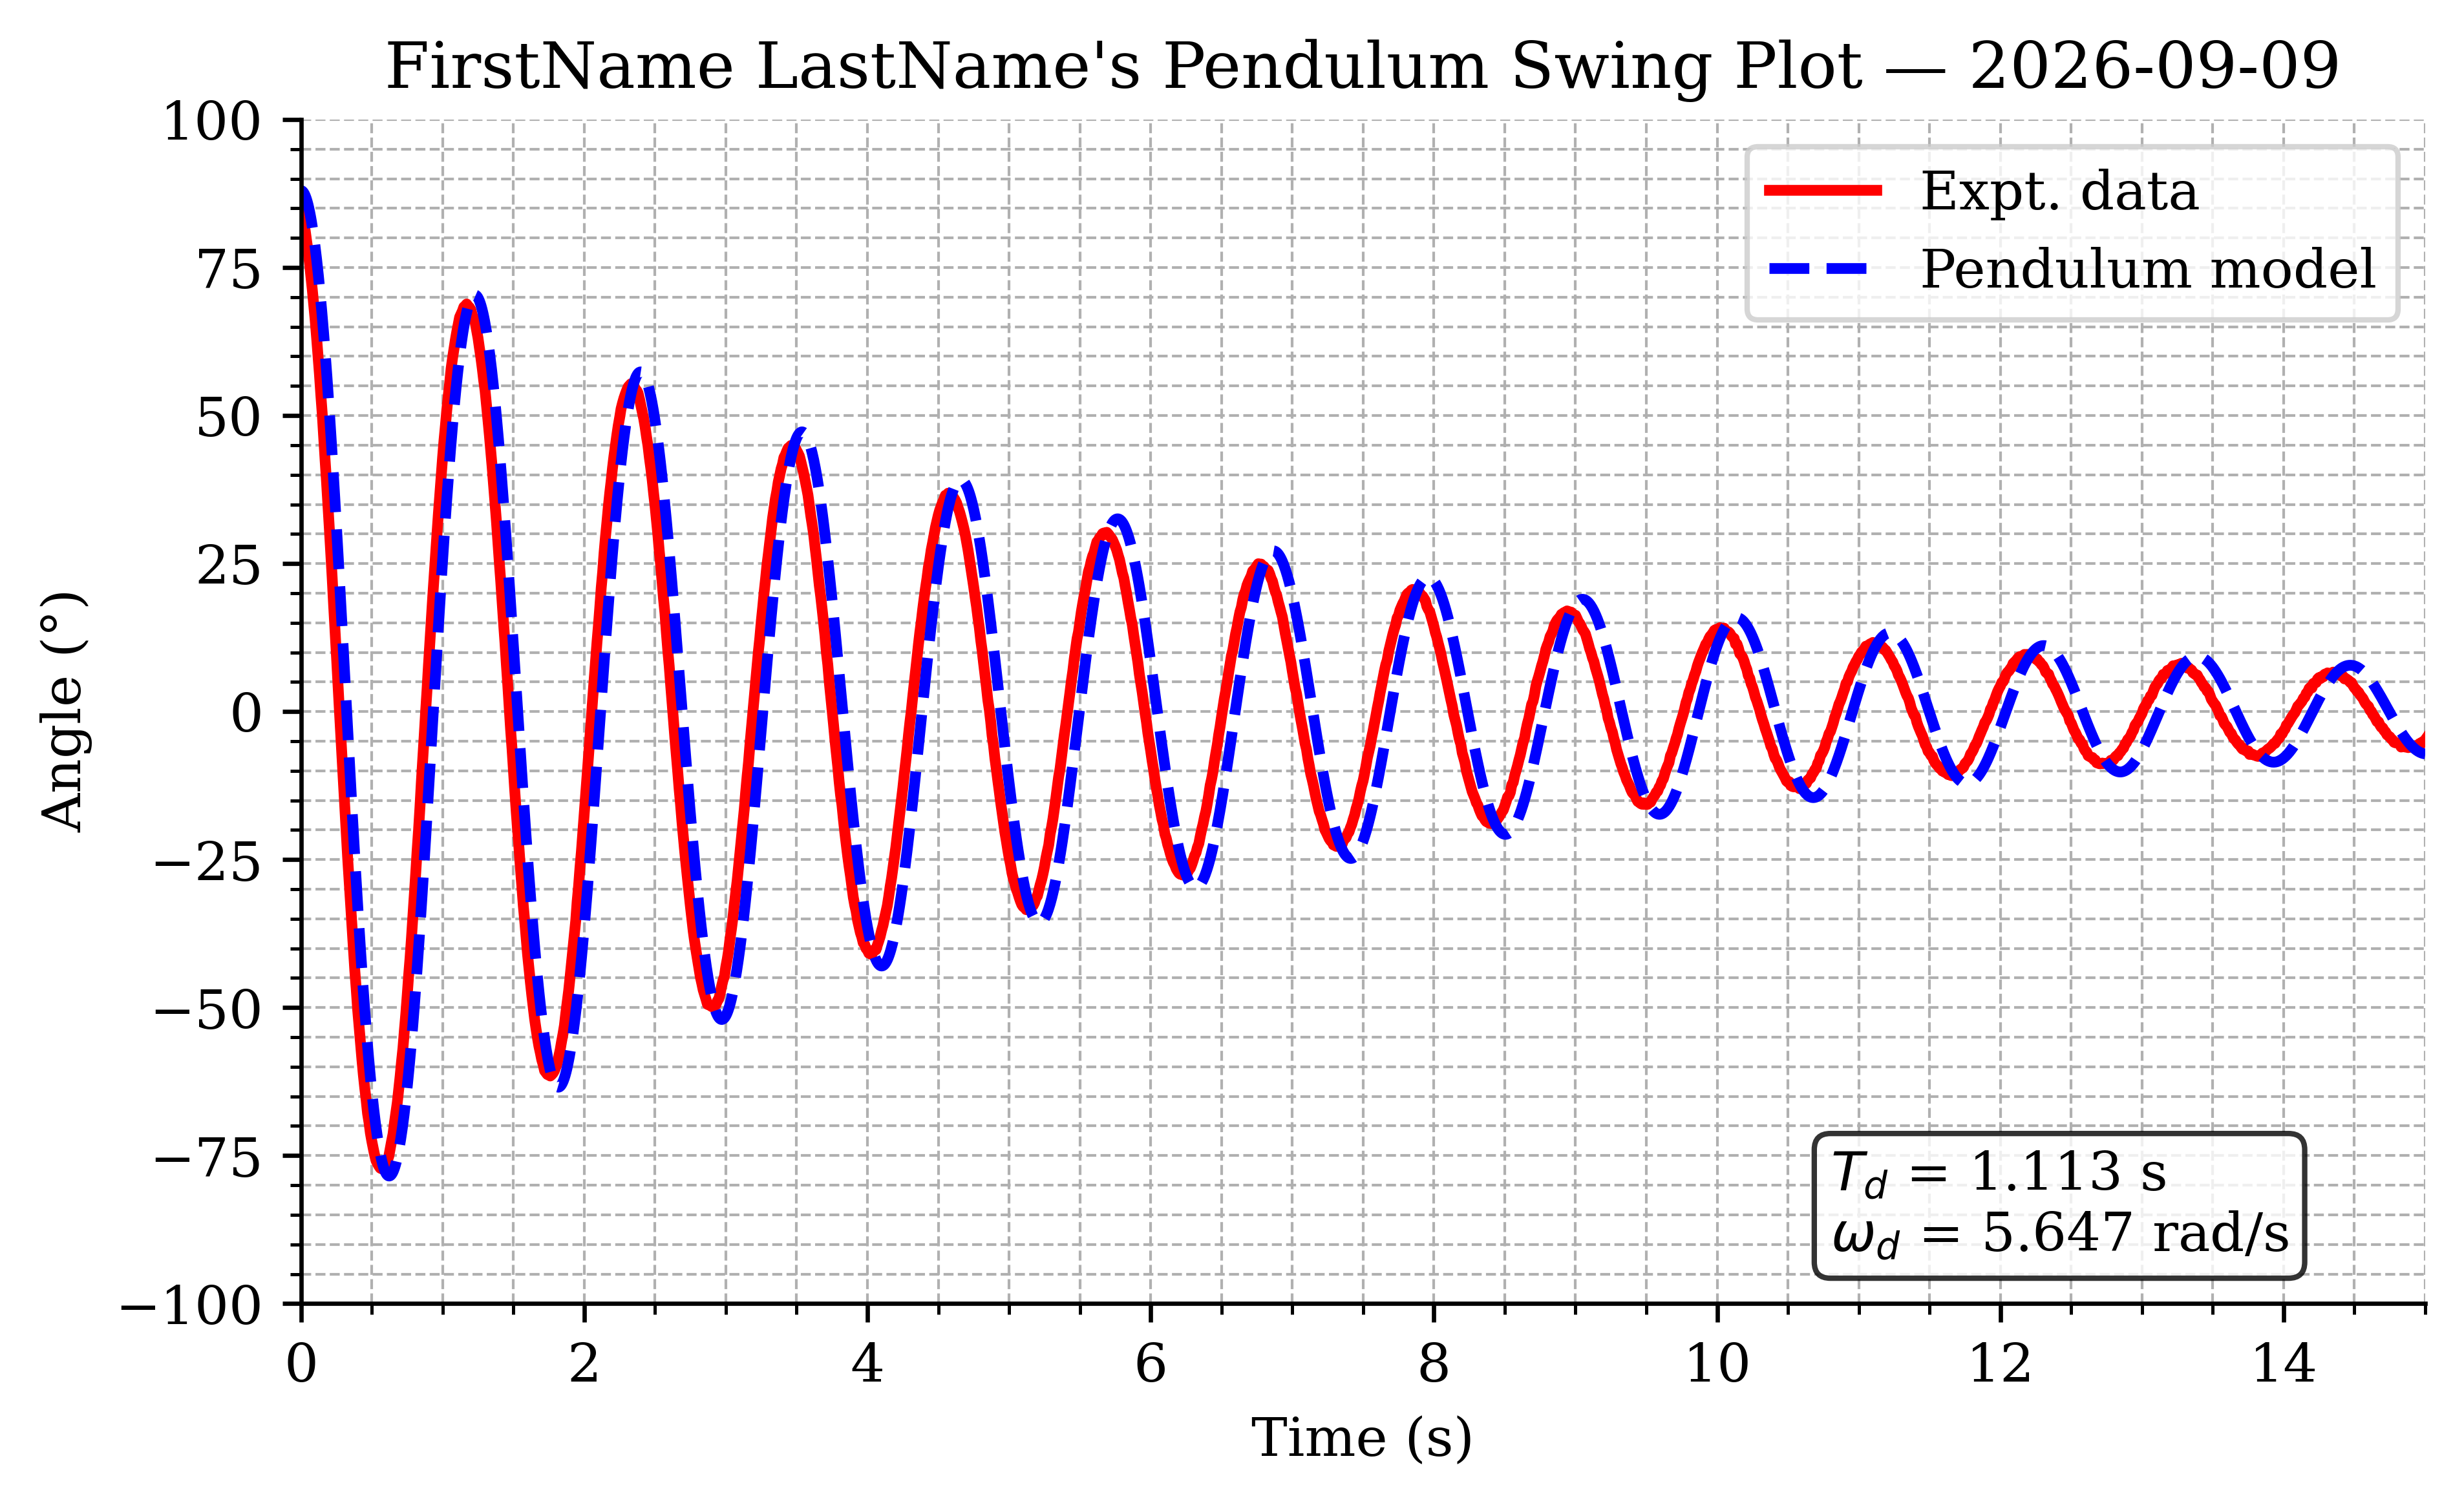
\includegraphics[width=6.5in,height=\textheight,keepaspectratio]{figures/Python/FirstName_LastName_Lab02_Swing.png}

}

\caption{\label{fig-example-swing}Example pendulum swing plot with tuned
model overlay (made-up data). Your values will differ, but your
formatting and annotations should match.}

\end{figure}%

\newpage{}

\section{Post-Lab Assignment}\label{post-lab-assignment}

Following the lab, upload your submissions to Canvas.
\ul{\textbf{Post-labs are due Mondays at 10:00 pm.}} A full example
solution notebook will be posted after all lab sections have met --- use
it to check your approach, but the work you submit must be your own.

\subsection{Submission Items}\label{submission-items}

\begin{itemize}
\tightlist
\item
  Your final \textbf{.ipynb} notebook file
  (\texttt{FirstName\_LastName\_Lab02.ipynb}), restarted and run
  top-to-bottom
\item
  Your calibration plot in \textbf{.pdf} format
\item
  Your pendulum swing plot with model overlay in \textbf{.pdf} format
\item
  Answers to the post-lab questions on Canvas
\end{itemize}

\subsection{Calibration Plot
Requirements}\label{calibration-plot-requirements}

\begin{itemize}
\tightlist
\item
  Figure size: 6.5'' wide × 4.0'' tall; white background
\item
  All text in Times font; 10--12 pt
\item
  Major and minor grids on; top and right spines removed
\item
  Calibration data: red circle markers, size 75
\item
  Linear fit: solid blue line, 2 pt
\item
  95\% CI lines: dashed black, 1 pt
\item
  Legend placed so it does not cover data
\item
  Axis labels with units; title ``FirstName LastName's Calibration
  Plot'' with the date
\item
  Text annotation (via \texttt{ax.text}, 4 decimal places, with units):
  calibration equation, norm of residuals, \(s_{yx}\), and \(S_{a_1}\)
\end{itemize}

\subsection{Swing Plot Requirements}\label{swing-plot-requirements}

\begin{itemize}
\tightlist
\item
  Figure size: 6.5'' wide × 4.0'' tall; white background
\item
  All text in Times font; 10--12 pt
\item
  Major and minor grids on; top and right spines removed
\item
  Experimental data: solid red line, 2 pt
\item
  Tuned model: dashed blue line, 2 pt
\item
  Time axis starts at the release (\(t = 0\)); set y-limits to about
  ±100°
\item
  Legend, axis labels with units; title ``FirstName LastName's Pendulum
  Swing Plot'' with the date
\item
  Text annotation (via \texttt{ax.text}): measured \(T_d\) (s) and
  \(\omega_d\) (rad/s)
\end{itemize}

\subsection{Post-Lab Questions}\label{post-lab-questions}

Be prepared to answer the following (make sure you can answer these
before leaving lab!):

\begin{enumerate}
\def\labelenumi{\arabic{enumi}.}
\tightlist
\item
  Report your calibration equation, with units on both coefficients.
\item
  What are your norm of residuals and \(s_{yx}\)? What do they tell you
  about your calibration quality?
\item
  What values of \texttt{L}, \texttt{zeta}, and \texttt{theta0} gave the
  best model agreement? How does the tuned \texttt{L} compare to your
  measured length?
\item
  Give two physical reasons why the simple pendulum model deviates from
  your measured data.
\end{enumerate}

\section{Before you leave}\label{before-you-leave}

\begin{itemize}
\tightlist
\item
  Remove all jumper wires from the breadboard and return them to the
  wire bin, sorted by color; discard any damaged wires.
\item
  Disconnect the pendulum leads and set the apparatus back at its
  station.
\item
  Return the DMM, protractor, and tools to their designated locations.
\item
  Confirm your data files have finished syncing to OneDrive --- check on
  your phone or a second device.
\item
  Make sure \textbf{both} partners have access to all data files and the
  notebook.
\item
  Make sure the station is clean, collect your belongings, and log off
  the computer.
\end{itemize}




\end{document}
